% ============================================================
% Template de TCC (Artigo Científico) — Faculdade UCL
% Versão simplificada: documentclass "article" padrão, fonte
% Computer Modern (pdfLaTeX), sem formatação ABNT customizada
% (sem capa separada, títulos de seção em maiúsculas simples,
% autores centralizados com notas de rodapé numeradas, legendas
% de figura no padrão default do LaTeX ("Figure")).
%
% Compile com pdfLaTeX (não depende de fontspec/XeLaTeX).
% ============================================================
\documentclass[12pt,a4paper]{article}

\usepackage[a4paper,margin=2.5cm]{geometry}
\usepackage{graphicx}
\graphicspath{{../../../assets/}}
\usepackage{array}
\usepackage{xcolor}
\usepackage[alf]{abntex2cite}
\usepackage[colorinlistoftodos,textsize=footnotesize]{todonotes}
\usepackage{tikz}
\usetikzlibrary{arrows.meta,positioning}
\usepackage{longtable}
\renewcommand{\refname}{Referências}

% ---------- Comentários de revisão coloridos (inline, já existentes no artigo original) ----------
\newcommand{\revmudar}[1]{\todo[inline,color=red!25!white,bordercolor=red]{\textbf{MUDAR:} #1}}
\newcommand{\revbom}[1]{\todo[inline,color=green!25!white,bordercolor=green!60!black]{\textbf{FICOU BOM:} #1}}
\newcommand{\revfaltou}[1]{\todo[inline,color=yellow!35!white,bordercolor=orange]{\textbf{FALTOU DETALHE:} #1}}

% ---------- Camada de revisão da banca Banca_TCC ----------
% \grifo{...}       destaca (grifa, fundo amarelo) o trecho exato a que o comentário se refere.
% \parecerGrave{..} parecer de problema crítico/alto -- compromete rigor ou validade -- vermelho.
% \parecerAjuste{.} parecer de ajuste moderado/baixo, não bloqueante -- laranja.
% \parecerElogio{.} parecer de elogio com sugestão de refinamento -- azul.
% \parecerPergunta{} pergunta direta de banca -- roxo.
% \colorbox em vez de \soul{}\hl{} (pacote soul indisponível offline nesta máquina) -- por isso
% cada \grifo{} deve envolver só um trecho curto (até ~1 linha), nunca um parágrafo inteiro: um
% \colorbox não quebra entre linhas.
\newcommand{\grifo}[1]{\colorbox{yellow}{#1}}
\newcommand{\parecerGrave}[1]{\todo[inline,color=red!10!white,bordercolor=red!70!black]{%
  \textbf{\color{red!60!black}BANCA\_TCC -- PROBLEMA CRÍTICO/ALTO:} #1}}
\newcommand{\parecerAjuste}[1]{\todo[inline,color=orange!12!white,bordercolor=orange!80!black]{%
  \textbf{\color{orange!70!black}BANCA\_TCC -- AJUSTAR:} #1}}
\newcommand{\parecerElogio}[1]{\todo[inline,color=blue!8!white,bordercolor=blue!60!black]{%
  \textbf{\color{blue!50!black}BANCA\_TCC -- BOM, MAS PODE MELHORAR:} #1}}
\newcommand{\parecerPergunta}[1]{\todo[inline,color=violet!10!white,bordercolor=violet]{%
  \textbf{\color{violet}A BANCA VAI PERGUNTAR:} #1}}

\setlength{\parindent}{0pt}
\setlength{\parskip}{0.8em}

% Identificadores \texttt{} longos sem ponto de quebra natural -- tolerância
% maior evita overfull hbox extrapolando a margem.
\tolerance=9999
\emergencystretch=3em
\hbadness=10000

% ---------- Numeração de página no canto superior direito ----------
\makeatletter
\def\ps@ucl{%
  \def\@oddhead{\hfil\normalfont\thepage}%
  \def\@evenhead{\hfil\normalfont\thepage}%
  \def\@oddfoot{}%
  \def\@evenfoot{}%
}
\makeatother
\pagestyle{ucl}

\begin{document}

\begin{center}
\fbox{\parbox{0.92\textwidth}{
\textbf{NOTA SOBRE ESTA VERSÃO}\\[0.3em]
Este é o arquivo \texttt{artigo\_revisado.tex} -- cópia do \texttt{Artigo.tex} atual, com uma
camada adicional de revisão gerada pelo agente \textbf{Banca\_TCC} (parecer completo em
\texttt{Parecer\_Banca\_TCC.pdf}, nota geral $\approx 6{,}33/10$). Os problemas apontados aparecem
em caixas \textbf{\color{red!60!black}vermelhas} (crítico/alto -- compromete rigor ou validade,
resolver antes da entrega) e \textbf{\color{orange!70!black}laranjas} (ajuste moderado/baixo, não
bloqueante). O trecho exato a que cada parecer se refere aparece \grifo{grifado em amarelo} logo
antes do comentário. O veredito final e a tabela de ações priorizadas estão na última seção, antes
das referências.
}}
\end{center}

\clearpage

% ============================================================
% PÁGINA 1 — cabeçalho, título, autores, resumo
% ============================================================
\thispagestyle{ucl}

\begin{center}
    
\includegraphics[width=3.6cm]{logo_ucl.png}\\[1em]

    Trabalho de Conclusão de Curso de Engenharia da Computação\\[0.8em]

    \textbf{\MakeUppercase{RadarTorres}:}\\
    \MakeUppercase{protótipo para detecção, localização e seleção automática de torre com controlador heurístico-neuroevolutivo}\\[0.8em]

    \textbf{\itshape RadarTorres:}\\
    \itshape a prototype for target detection, localization and automatic tower selection with a heuristic-neuroevolutionary controller\\[1.2em]
\end{center}

\begin{center}
    Gabriel Vasconcellos de Morais\footnote{Graduando(a) em Engenharia da Computação pela Faculdade do Centro Leste -- UCL. E-\textit{mail}: gabrielmorais@ucl.br}\\
    Matheus Emanoel Gomes Souza\footnote{Graduando(a) em Engenharia da Computação pela Faculdade do Centro Leste -- UCL. E-\textit{mail}: matheusemanoel@ucl.br}\\
    Anker Douglas Loss\footnote{Orientador(a). \grifo{Mestre em xxx pela xxx}. E-\textit{mail}: anker@ucl.br}
\end{center}

\parecerAjuste{Placeholder não preenchido ("Mestre em xxx pela xxx") no rodapé de identificação do
orientador -- ajuste de baixa gravidade, mas deve ser preenchido antes de qualquer submissão
formal.}

\begin{center}
    \textbf{RESUMO}
\end{center}

\noindent A construção de protótipos de sensoriamento com hardware acessível é um recurso
didático relevante em Engenharia da Computação, por permitir explorar de forma prática conceitos
de aquisição de dados, rastreamento e tomada de decisão automática. Este trabalho apresenta o
RadarTorres, um protótipo que detecta um alvo em movimento, estima sua posição e decide, entre um
conjunto de torres candidatas posicionadas ao redor de uma base central, qual delas deve responder
a esse alvo -- problema central que o trabalho busca resolver: como identificar, localizar e
atribuir automaticamente a torre mais adequada a cada alvo, de forma auditável e sem depender de
sensores ou atuadores de uso industrial. O sistema combina dois sensores ultrassônicos (que medem
a distância pelo eco do ultrassom) com \grifo{quatro câmeras de 720p}, processa quadros de vídeo
(\textit{frames}) e classifica o alvo por sua cor, formato e tamanho. O protótipo converte as
leituras de ângulo e distância em posição cartesiana, exibindo-as em tempo real em um radar
circular, seleciona automaticamente a torre mais adequada para cada alvo e registra em auditoria
toda ação executada. Essa seleção combina uma heurística determinística, escrita como regras
explícitas de engenharia, com uma rede neural que aprende, por meio de um algoritmo genético
próprio, a refinar essa escolha e o instante do acionamento. O treinamento dessa rede ocorre
inteiramente antes da operação do sistema, em um ambiente simulado que executa gerações de
episódios de teste até evoluir os parâmetros da rede; concluído o treinamento, esses parâmetros
são incorporados de forma fixa à aplicação, de modo que, durante a execução real, o sistema apenas
aplica o que foi aprendido previamente, sem ajustar seus parâmetros em tempo real. O processamento
e a tomada de decisão são concentrados em uma aplicação desktop, com arquitetura pensada para
permitir evolução futura sem exigir hardware adicional. Discutem-se, por fim, as limitações
inerentes à abordagem de hardware acessível e de baixo custo adotada, e o fato de a validação do
protótipo, até o momento, ter sido realizada inteiramente por simulação de software, já que a
estrutura física ainda não foi montada nem testada.

\parecerAjuste{O número de câmeras (quatro) e a resolução (720p), citados aqui e na Seção 2.3.3,
não têm registro no código nem na documentação técnica do repositório (o próprio \texttt{.tex}
fonte marca isso com um comentário "CONFIRMAR" não renderizado no PDF). Decida se é uma decisão de
projeto já tomada ou uma aspiração ainda não implementada, e torne essa distinção visível ao leitor
do PDF -- hoje ela só existe em comentário de fonte.}

\noindent\textbf{Palavras-chave}: Detecção e rastreamento de alvos; Seleção automática de torre; Controlador heurístico-neuroevolutivo; Arduino; Protótipo.

\begin{center}
    \textbf{ABSTRACT}
\end{center}

\noindent This work presents RadarTorres, a prototype developed as a Final Course Project in
Computer Engineering that detects a moving target, estimates its position, and decides, among a
set of candidate towers placed around a central base, which one should respond to that target --
the central problem this work addresses: how to automatically identify, localize, and assign the
most suitable tower to each target, in an auditable way and without relying on industrial-grade
sensors or actuators. The system combines two ultrasonic sensors (which measure distance by
ultrasound echo) with four 720p cameras, processes video frames, and classifies the target by
color, shape, and size. The prototype converts angle and distance readings into Cartesian
position, displaying them in real time on a circular radar, automatically selects the most
suitable tower for each target, and logs every executed action for auditing. This selection
combines a deterministic heuristic, written as explicit engineering rules, with a neural network
that learns, through a custom genetic algorithm, to refine that choice and the activation timing.
Training of this network happens entirely before the system is put into operation, in a simulated
environment that runs generations of test episodes until the network's parameters evolve; once
training is complete, these parameters are embedded as fixed values into the application, so
that, during actual execution, the system only applies what was previously learned, without
adjusting its parameters in real time. Processing and decision-making are concentrated in a
desktop application, with an architecture designed to allow future evolution without requiring
additional hardware. Finally, the limitations inherent to the accessible, low-cost hardware
approach adopted are discussed, as is the fact that validation of the prototype has so far been
carried out entirely through software simulation, since the physical structure has not yet been
assembled or tested.

\noindent\textbf{Keywords}: Target detection and tracking; Automatic tower selection; Heuristic-neuroevolutionary controller; Arduino; Prototype.

\clearpage

% ============================================================
% 1 INTRODUÇÃO
% ============================================================
\section{Introdução}

Sistemas automáticos de detecção e resposta a alvos exigem, além de identificar um estímulo,
rastrear com precisão sua posição e aplicar regras de decisão que evitem respostas indevidas --
tarefas comumente resolvidas com sensores de radar, de custo elevado. Como alternativa a esse tipo
de equipamento, este trabalho adota técnicas de visão computacional, aliadas a hardware acessível,
como parte central da arquitetura do protótipo. Protótipos didáticos construídos dessa forma
desempenham papel importante nesse processo, por permitirem que esses conceitos sejam explorados
de forma prática e replicável em laboratório, reproduzindo os princípios de sensoriamento,
rastreamento e decisão presentes em sistemas mais sofisticados.

O protótipo resultante, denominado RadarTorres, combina sensores ultrassônicos e câmeras para
detectar um alvo, estimar sua posição em um radar circular e decidir, entre um conjunto de torres
candidatas dispostas ao redor de uma base central, qual delas deve responder a esse alvo. Essa
decisão não é tomada apenas por regras fixas: uma rede neural, evoluída por um algoritmo genético
próprio, aprende a refinar a escolha da torre e o instante do acionamento, sempre dentro dos
limites que uma camada de regras explícitas (a heurística) já considera seguros. Esse aprendizado
acontece em duas etapas bem separadas: antes da operação do sistema, em um ambiente de treinamento
simulado, onde a rede evolui ao longo de muitas gerações de episódios de teste; e, depois de
treinada, apenas na forma de inferência durante a execução real, sem qualquer ajuste adicional de
seus parâmetros em tempo de operação. O problema central que este trabalho busca resolver é,
portanto, como automatizar essa cadeia -- detectar, localizar e selecionar a torre mais adequada a
cada alvo -- de forma auditável e \grifo{replicável em laboratório}, sem depender de sensores ou atuadores
de uso industrial.

\parecerAjuste{"Replicável em laboratório" é parte da formulação do próprio problema de pesquisa,
mas nenhuma replicação em bancada física foi de fato realizada -- toda validação relatada no
trabalho é por simulação de software (ver Seção 2.2). O trabalho é auditável no sentido de
rastreabilidade de código/decisão, mas a "replicabilidade em laboratório" permanece não
demonstrada. Sugestão: reformular para algo como "...de forma auditável e, no estágio atual do
projeto, com arquitetura concebida para replicação futura em laboratório...", deixando claro que é
uma propriedade de projeto, não um resultado obtido.}

% ============================================================
% 2 DESENVOLVIMENTO
% ============================================================
\section{Desenvolvimento}

\subsection{Revisão da literatura e fundamentação teórica}

Sistemas de detecção e rastreamento de alvos costumam recorrer a sensores como radar, de custo
elevado. Como alternativa, sensores acessíveis podem ser combinados de modo que as limitações de
um sejam compensadas pelas qualidades do outro. Sensores ultrassônicos, como o HC-SR04, medem
distância com boa confiabilidade em curto alcance, mas não distinguem o tipo do obstáculo;
câmeras, por sua vez, fornecem informação semântica, porém dependem das condições de iluminação e
exigem maior poder de processamento \cite{majoni2025}. A fusão de sensores (\textit{sensor
fusion}) combina as duas modalidades para aproveitar essa complementaridade.

\citeonline{majoni2025} descrevem uma arquitetura em que um Arduino Mega trata o sensoriamento
ultrassônico de baixa latência, enquanto um Raspberry Pi processa as imagens da câmera com uma rede
YOLOv4-tiny, com comunicação serial entre os dois. Essa divisão de papéis é análoga à do
RadarTorres, em que o Arduino realiza a aquisição e a aplicação desktop concentra o processamento.

A literatura também mostra que sensores ultrassônicos acessíveis podem complementar outras fontes
de sensoriamento em sistemas de rastreamento, com a precisão melhorada por predição baseada em
filtro de Kalman e fusão com a distância medida pelos ultrassônicos \cite{curbscan}. O mesmo trabalho observa
que as leituras ultrassônicas se tornam ruidosas em distâncias maiores, o que motiva o uso de
filtragem.

Definidos o alvo e sua posição, resta decidir qual recurso deve responder. Na literatura de defesa,
esse problema é tratado como avaliação de ameaças e atribuição de armas (\textit{Threat Evaluation
and Weapon Assignment}, TEWA), no qual as informações dos sensores alimentam as etapas de detecção,
rastreamento e identificação, seguidas da avaliação da ameaça e da atribuição dos recursos. As
abordagens desse tipo de problema costumam ser classificadas em ameaça por ameaça, em que os
recursos são atribuídos sequencialmente, e multiameaça, em que o conjunto de ameaças é considerado
simultaneamente.

O RadarTorres adota uma abordagem simples, por proximidade, aplicada alvo a alvo, com propósito
exclusivamente demonstrativo (laser de baixa potência, LED ou simulação, sem armamento real); a
abordagem multiameaça fica como trabalho futuro.

O refinamento dessa escolha por proximidade -- e o instante de disparo -- é feito por uma pequena
rede neural \textit{feedforward} (7 entradas, 1 camada oculta de 8 neurônios, 2 saídas, ativação
tanh), cujos pesos não são ajustados por retropropagação, mas evoluídos por um algoritmo genético
próprio (seleção por torneio, \textit{crossover} uniforme, mutação gaussiana, elitismo), auditável e
sem dependência de biblioteca de aprendizado de máquina. \citeonline{such2017deepneuroevolution}
mostram que algoritmos genéticos são uma alternativa competitiva ao treino por gradiente em tarefas
de aprendizado por reforço, em redes de porte bem maior do que a aqui empregada (até quatro milhões
de parâmetros, contra os 82 parâmetros da rede do RadarTorres). Esse resultado sustenta a escolha
do algoritmo genético como método de treinamento, mas não implica, por si só, que aumentar o número
de camadas ou neurônios seja desnecessário; por isso, a estratégia adotada para ampliar o
desempenho do controlador prioriza o ajuste dos hiperparâmetros da busca evolutiva (tamanho de
população, paralelização da avaliação de fitness, enriquecimento do sinal de recompensa), sem
descartar, a priori, uma rede maior caso evidências futuras mostrem que a capacidade atual seja o
fator limitante.

\parecerElogio{Esta é a melhor seção do artigo: cada citação (Such et al. 2017, Huang \& Ontañón
2020 mais abaixo) é amarrada explicitamente a uma decisão de projeto concreta, em vez de citada de
passagem. As duas citações mais centrais foram verificadas pela banca em busca externa e a
representação do artigo é fiel ao conteúdo original -- ver Seção F do parecer. Ponto a melhorar:
a base bibliográfica é estreita (7 referências) para um TCC desta extensão.}

A arquitetura híbrida do controlador -- heurística que restringe o espaço de ações antes da rede
decidir, e volta a intervir depois, vetando o disparo -- tem paralelo direto com duas técnicas da
literatura de aprendizado por reforço. A primeira é o mascaramento de ações inválidas
(\textit{action masking}): \citeonline{huang2020actionmasking} mostram, para algoritmos de
gradiente de política, que mascarar o espaço de ações antes da amostragem corresponde a uma
atualização de gradiente válida e se torna mais importante quanto maior a fração de ações
inválidas -- o que justifica tecnicamente a etapa em que a camada heurística do RadarTorres
restringe as torres candidatas (nunca ocupada, nunca fora de alcance) antes de a rede neural
escolher entre elas. A segunda é o \textit{shielding}: \citeonline{alshiekh2017shielding} propõem
um componente reativo (\textit{shield}) que intercepta a ação escolhida pela política aprendida e a
substitui quando ela violaria uma propriedade de segurança expressa em lógica temporal -- papel
equivalente ao do veto heurístico final do RadarTorres sobre o disparo, que nunca é delegado à
rede. A atribuição de recursos defensivos a ameaças, por sua vez, é tratada na literatura de TEWA
tanto no caso ameaça por ameaça quanto no caso multiameaça \cite{tewa2009,tewa_multiameaca2009};
o RadarTorres adota deliberadamente a abordagem mais simples (proximidade, alvo a alvo), com a
multiameaça permanecendo como trabalho futuro já apontado anteriormente.

O impacto do treinamento virtual sobre a execução física do controlador é atenuado por uma decisão
de projeto central: o mesmo controlador híbrido -- heurística e rede neural combinadas -- que
decide no episódio simulado é o que decide em produção, consultado pelo algoritmo responsável por
selecionar a torre a partir das leituras do Arduino real -- não há conversão para um formato
intermediário (ONNX, TensorFlow Lite) nem reimplementação em outra linguagem ou plataforma, fontes
comuns de divergência entre o comportamento treinado e o executado em sistemas de aprendizado por
reforço aplicados a robótica. O genoma evoluído é um vetor plano de pesos e vieses, embutido
diretamente na aplicação por uma etapa automática de build, que grava o melhor genoma treinado no
executável, de onde é carregado por um componente dedicado em tempo de execução; o que muda do
ambiente de treino para a operação real é apenas a origem dos dados de entrada (leitura simulada
ou leitura do Arduino), nunca a função de decisão em si. Os parâmetros que definem o episódio
simulado -- alcance de engajamento e certeza mínima para autorizar disparo -- também deixaram de
ser constantes fixas no código e passaram a ser lidos das mesmas configurações de alcance de mira
e de limiar de certeza usadas pelo sistema real, de modo que recalibrar o alcance da câmera ou o
limiar de certeza no painel de Configurações recalibra também o mundo de treino, reduzindo a
divergência entre o que foi aprendido e o que será executado. Por fim, a rede neural nunca decide
isoladamente: ela apenas pondera a escolha dentro do que a camada heurística determinística já
considera válida (nunca uma torre ocupada, nunca fora de alcance), de modo que a arquitetura foi
concebida para limitar o pior caso de uma generalização imperfeita do treino virtual para a física
-- no limite, o controlador regrediria ao comportamento puramente heurístico, nunca a uma decisão
arbitrária; trata-se, porém, de uma propriedade de projeto ainda não submetida a validação em
hardware físico real.

% PREENCHER: referência sobre classificação de objetos por cor, formato e tamanho em visão
% computacional clássica (a ser informada pelo autor).

\parecerAjuste{O próprio \texttt{.tex} fonte contém, neste ponto, um comentário não renderizado
"PREENCHER: referência sobre classificação de objetos por cor, formato e tamanho" -- uma lacuna
teórica central (o módulo de visão, Seção 2.3.3, depende exatamente dessa técnica) ainda sem
citação. Resolver antes da entrega.}

\subsection{Procedimentos metodológicos}
\label{sec:procedimentos-metodologicos}

O percurso metodológico deste trabalho não seguiu o fluxo tradicional de especificação prévia
seguida de implementação: o protótipo RadarTorres já existia, em desenvolvimento incremental,
antes do levantamento formal de requisitos. Optou-se, portanto, por catalogar os requisitos
funcionais e não funcionais diretamente a partir do que já estava implementado no código-fonte da
aplicação desktop e da documentação técnica já produzida ao longo do projeto, em vez de defini-los
a priori em um documento de especificação anterior à codificação. O treinamento do controlador por
neuroevolução, descrito na Seção 2.1, segue essa mesma lógica incremental: a arquitetura híbrida
heurística+rede neural foi definida e ajustada em paralelo ao restante do sistema, não a partir de
um plano de treinamento fechado desde o início.

Esse levantamento resultou em 25 requisitos funcionais (RF01--RF25) e 20 requisitos não
funcionais (RNF01--RNF20), classificados segundo dois critérios objetivos: a \textbf{prioridade},
atribuída conforme a criticidade de cada requisito para a operação central do sistema
(comunicação serial, rastreamento, seleção de torre, modos de operação e segurança recebem
prioridade Alta; suporte administrativo e ferramental, Média; conveniências de interface, Baixa);
e o \textbf{status}, que reflete o estado real de implementação constatado no código no momento do
levantamento -- Implementado, Parcial ou Planejado --, e não a intenção original de projeto. Cada
requisito foi, além disso, rastreado até a classe ou método do código-fonte que o realiza, registro
mantido em uma matriz de rastreabilidade dedicada, de modo que qualquer afirmação sobre o grau de
implementação do protótipo possa ser \grifo{verificada diretamente no código}. Divergências encontradas
entre o comportamento observado no código e a nomenclatura ou fluxo originalmente esperado também
foram registradas explicitamente, em vez de omitidas ou corrigidas silenciosamente na
documentação.

\parecerGrave{Esta alegação de rastreabilidade total é contradita pelas próprias Seções 2.3.2 e
2.3.3: os comentários "CONFIRMAR" do \texttt{.tex} fonte admitem que o conteúdo sobre motores,
drivers, registradores, dimensões, número de câmeras e resolução "foi informado pelo autor e ainda
não consta da documentação técnica do repositório", e em alguns casos contradiz
\texttt{Diagrama\_Eletrico.md}. Essa divergência entre o método declarado e o método efetivamente
aplicado em parte do texto é o problema crítico mais importante deste parecer -- ver Seções C e E.}

\textbf{A parte física do RadarTorres (torres, motores, sensores montados em campo) ainda não foi
implementada nem validada.} Toda a validação funcional relatada neste trabalho foi realizada por
simulação de software: a lógica de rastreamento de alvos e de seleção automática de torre foi
exercitada de ponta a ponta sem depender de uma porta serial conectada a hardware real, o que
impõe um limite claro ao escopo dos resultados relatados -- eles atestam a corretude da lógica de
decisão implementada em software, mas não substituem uma validação de campo com sensores e torres
físicas, deixada como trabalho futuro.

\parecerElogio{Declaração de limitação exemplarmente honesta e reiterada de forma consistente do
resumo à conclusão -- mérito metodológico incomum em TCCs de graduação.}

A mesma ressalva se aplica, com reforço adicional, ao controlador treinado por neuroevolução: o
mundo simulado em que os genomas são avaliados é uma aproximação
idealizada do ambiente físico -- os alvos nascem na borda de um círculo e avançam de forma quase
radial, sem o ruído típico de leituras ultrassônicas reais; a certeza de identificação do alvo pela
câmera é modelada como uma função sintética que cresce com o tempo de observação, e a probabilidade
de errar o disparo é uma função assumida, crescente com a velocidade do alvo -- nenhuma delas
calibrada com dados de campo, já que o hardware ainda não foi montado. Essa distância entre
simulação e realidade física não é apenas teórica: durante este trabalho, identificou-se e
corrigiu-se uma falha em que a certeza de identificação do alvo era sorteada uma única vez, no
nascimento, e nunca era atualizada -- cerca de 70\% dos alvos simulados nasciam permanentemente
abaixo do limiar mínimo de disparo e jamais podiam ser abatidos, independentemente da qualidade do
genoma, mascarando qualquer evolução real do controlador sob a aparência de estagnação. O episódio
é citado aqui como evidência concreta de que uma premissa equivocada na simulação pode invalidar
silenciosamente o processo de treinamento sem que isso seja percebido pelas métricas agregadas,
reforçando a necessidade de validação cruzada entre o comportamento do genoma treinado e o
comportamento observado em campo, com hardware físico, antes de se confiar no controlador em um
cenário de operação real -- validação que permanece como trabalho futuro, nos mesmos termos já
apontados para o restante do protótipo.


A Tabela~\ref{tab:fitness-antes-depois} quantifica o achado, a partir do histórico de treinamento
persistido localmente (\texttt{historico\_treinamento\_geracoes} e
\texttt{marcos\_fitness\_treinamento}, tabelas descritas na Seção~\ref{sec:modelo-dados}). Antes da
correção (commit \texttt{a02d46a}), o fitness médio da população permaneceu estagnado em torno de 9
ao longo de 51 blocos de 500 gerações (25.500 gerações treinadas, entre 13h40 e 14h57 do mesmo dia),
mesmo com o melhor indivíduo de cada bloco oscilando entre 98 e 145 -- sinal de que indivíduos
pontualmente sortudos conseguiam boa pontuação, sem que a população como um todo convergisse,
exatamente o efeito esperado de 70\% dos alvos nascerem abaixo do limiar de disparo. Depois da
correção, a taxa de cobertura (fração de alvos que chegam a ser disparáveis) sobe para 100\% em
todas as cinco amostras de comportamento do melhor indivíduo registradas na mesma tarde, e o
fitness médio da população em uma amostra recente de 300 gerações (27/10, gerações 1141--1440) sobe
para 134,17, muito mais próximo do fitness do melhor indivíduo (137,35) do que o patamar de 9
observado antes da correção. O genoma embutido no executável (\texttt{genoma-controlador.json})
corresponde à geração 159, com \texttt{MelhorFitness} = 188,47.

\begin{table}[htbp]
  \centering
  \caption{Fitness da população antes e depois da correção do bug de certeza estática (commit
  \texttt{a02d46a}), a partir do histórico de treinamento persistido localmente.}
  \label{tab:fitness-antes-depois}
  \small
  \renewcommand{\arraystretch}{1.2}
  \begin{tabular}{p{4.6cm}p{3.6cm}p{3.6cm}}
    \hline
    \textbf{Métrica} & \textbf{Antes (bug)} & \textbf{Depois (corrigido)} \\
    \hline
    Fitness médio da população & $\approx$ 9,11 (min. 8,37, máx. 9,43; 51 blocos de 500 gerações) &
    134,17 (min. 121,31, máx. 150,60; amostra de 300 gerações) \\
    Melhor fitness por bloco/geração & 97,75 a 144,95 (média 119,62) & 137,35 em média
    (122,81 a 155,47) \\
    Taxa de cobertura dos alvos & não medida diretamente -- $\approx$ 70\% dos alvos
    permanentemente abaixo do limiar & 100\% (5/5 amostras pós-correção) \\
    Genoma embutido no executável & -- & geração 159, fitness 188,47 \\
    \hline
  \end{tabular}
\end{table}

\parecerAjuste{A célula "não medida diretamente -- $\approx$70\%" mistura, visualmente, uma
estimativa derivada com valores efetivamente medidos (que têm duas casas decimais de precisão).
Marque essa célula com uma nota de rodapé de tabela explícita, para o leitor não confundir
estimativa com medição.}

\subsection{Projeto e implementação}

\subsubsection{Módulo de detecção de alvos}

O módulo de detecção utiliza dois sensores ultrassônicos HC-SR04 instalados de costas um para o
outro no topo de um mastro, na torre central. O mastro é movido por um motor de passo 28BYJ-48 que
oscila 180°, de modo que, em conjunto, os dois sensores cobrem uma varredura de 360°. Cada sensor
emite pulsos de 40 kHz e calcula a distância pelo atraso do eco, segundo a relação
$d = \frac{v \cdot \Delta t}{2}$, em que $v$ é a velocidade do som no ar (cerca de 343 m/s à
temperatura ambiente). A cada leitura, o Arduino envia à aplicação desktop, pela porta serial, o
ângulo e a distância em protocolo de texto simples, que a aplicação converte em posição cartesiana
e exibe no radar circular de quatro quadrantes.

O protocolo é textual em ASCII, transportado pela porta serial USB a 9600 bauds por padrão, com
cada mensagem terminada por \texttt{\textbackslash n} e composta por um tipo em maiúsculas seguido
de pares chave-valor separados por ponto e vírgula. Uma leitura de alvo chega na forma
\texttt{TARGET;ID=1;ANGLE=45;DIST=2.80}, em que \texttt{ANGLE} é dado em graus no intervalo
$[0, 360)$ e \texttt{DIST} em metros. O ângulo segue a convenção de bússola -- $0^\circ$ apontando
para o Norte, sentido horário --, escolhida por ser a leitura mais intuitiva para quem opera um
radar, e a conversão para coordenadas cartesianas de mundo, feita por uma rotina dedicada de
conversão de coordenadas polares para cartesianas, é dada por $x = d \cdot \sin\theta$ e
$y = d \cdot \cos\theta$, com $\theta$ em radianos. A partir do par $(x, y)$, o quadrante do alvo é
determinado pelos sinais das duas coordenadas (por um algoritmo auxiliar de identificação de
quadrante) e a distância até cada torre candidata pela distância euclidiana clássica (calculada
por uma rotina dedicada de cálculo de distância). Leituras com
campos ausentes, não numéricos, com ângulo fora do intervalo válido ou com distância negativa são
convertidas em mensagens de erro registradas no console de eventos, nunca em exceções -- falhas de
sensor ou de cabo produzem degradação graciosa, e não interrupção da aplicação.

\subsubsection{Projeto elétrico e estrutural}

O projeto elétrico é baseado em um Arduino MEGA 2560 (ATmega2560, lógica 5V) -- substituiu um Arduino
Uno considerado em versão anterior do projeto, cujos ${\sim}20$ pinos não comportam os 13 motores de
passo da topologia atual. A varredura da torre central é feita por um motor de passo 28BYJ-48
acionado por um driver ULN2003; os outros nove eixos de mira (oito das quatro câmeras, em pan e
tilt, e quatro das torres armadas, só em pan) usam motores de passo NEMA17 com drivers
A4988/DRV8825, com um pino de habilitação (\textit{enable}) compartilhado entre os doze drivers.
Cada uma das quatro torres armadas possui, portanto, um único motor de pan (modelo 2D, sem tilt na
torre) e um laser de baixa potência como acionamento demonstrativo, sem indicador luminoso dedicado
-- a torre selecionada e o evento de disparo são sinalizados apenas via protocolo serial (mensagens
\texttt{ACK}/\texttt{STATUS}), não por LED. A alimentação dos doze drivers A4988/DRV8825 e do
ULN2003 (tensão e distribuição de terra) ainda não está especificada no firmware e permanece como
item a confirmar na montagem física. Na torre central, o mastro dos sensores não é acoplado
diretamente ao eixo do motor: ele assenta em um disco que gira sobre um rolamento axial 51108,
acionado pelo motor por um cubo duplo-D. A passagem dos fios fica próxima ao eixo central, com folga
de cabo em vez de anel coletor (\textit{slip ring}), já que o giro é limitado a 180°. A torre
central é cerca de 5 cm mais alta que as torres armadas (cerca de 137,5 mm de altura). As peças
estruturais são impressas em 3D, em formato de torre, com suporte para rolamento axial na base --
o que permite a rotação da estrutura --, comum às cinco torres. As torres armadas têm, além disso,
suportes próprios para o motor de pan e para as câmeras; a torre central tem suporte próprio para os
sensores ultrassônicos no topo do mastro. Todas essas peças, assim como o restante do projeto,
existem até o momento apenas em projeto digital (modelagem 3D e simulação elétrica), sem montagem
física realizada.

\parecerGrave{PROBLEMA CRÍTICO (ver Seção C.2 do parecer). O conteúdo grifado acima (Arduino Uno,
74HC595, ULN2003, fonte 5V/15A, rolamento 51108) é apresentado como fato assentado, sem qualquer
ressalva visível no PDF. Mas o próprio comentário "CONFIRMAR" do \texttt{.tex} fonte (não
renderizado) admite que esse conteúdo "foi informado pelo autor e ainda não consta da documentação
técnica do repositório", e que \texttt{Diagrama\_Eletrico.md} descreve um arranjo física e
eletricamente diferente (um HC-SR04, um servo SG90, quatro LEDs, alimentação pela USB). Isso
contradiz diretamente a alegação de rastreabilidade total ao código feita na Seção 2.2. Correção
sugerida: (a) atualizar \texttt{Diagrama\_Eletrico.md} para refletir o arranjo aqui descrito, OU
(b) inserir no corpo do PDF uma frase equivalente à já usada em outros pontos do artigo para
hardware não confirmado ("este arranjo existe até o momento apenas como especificação ainda não
reconciliada com a documentação técnica do projeto").}

\begin{figure}[htbp]
  \centering
  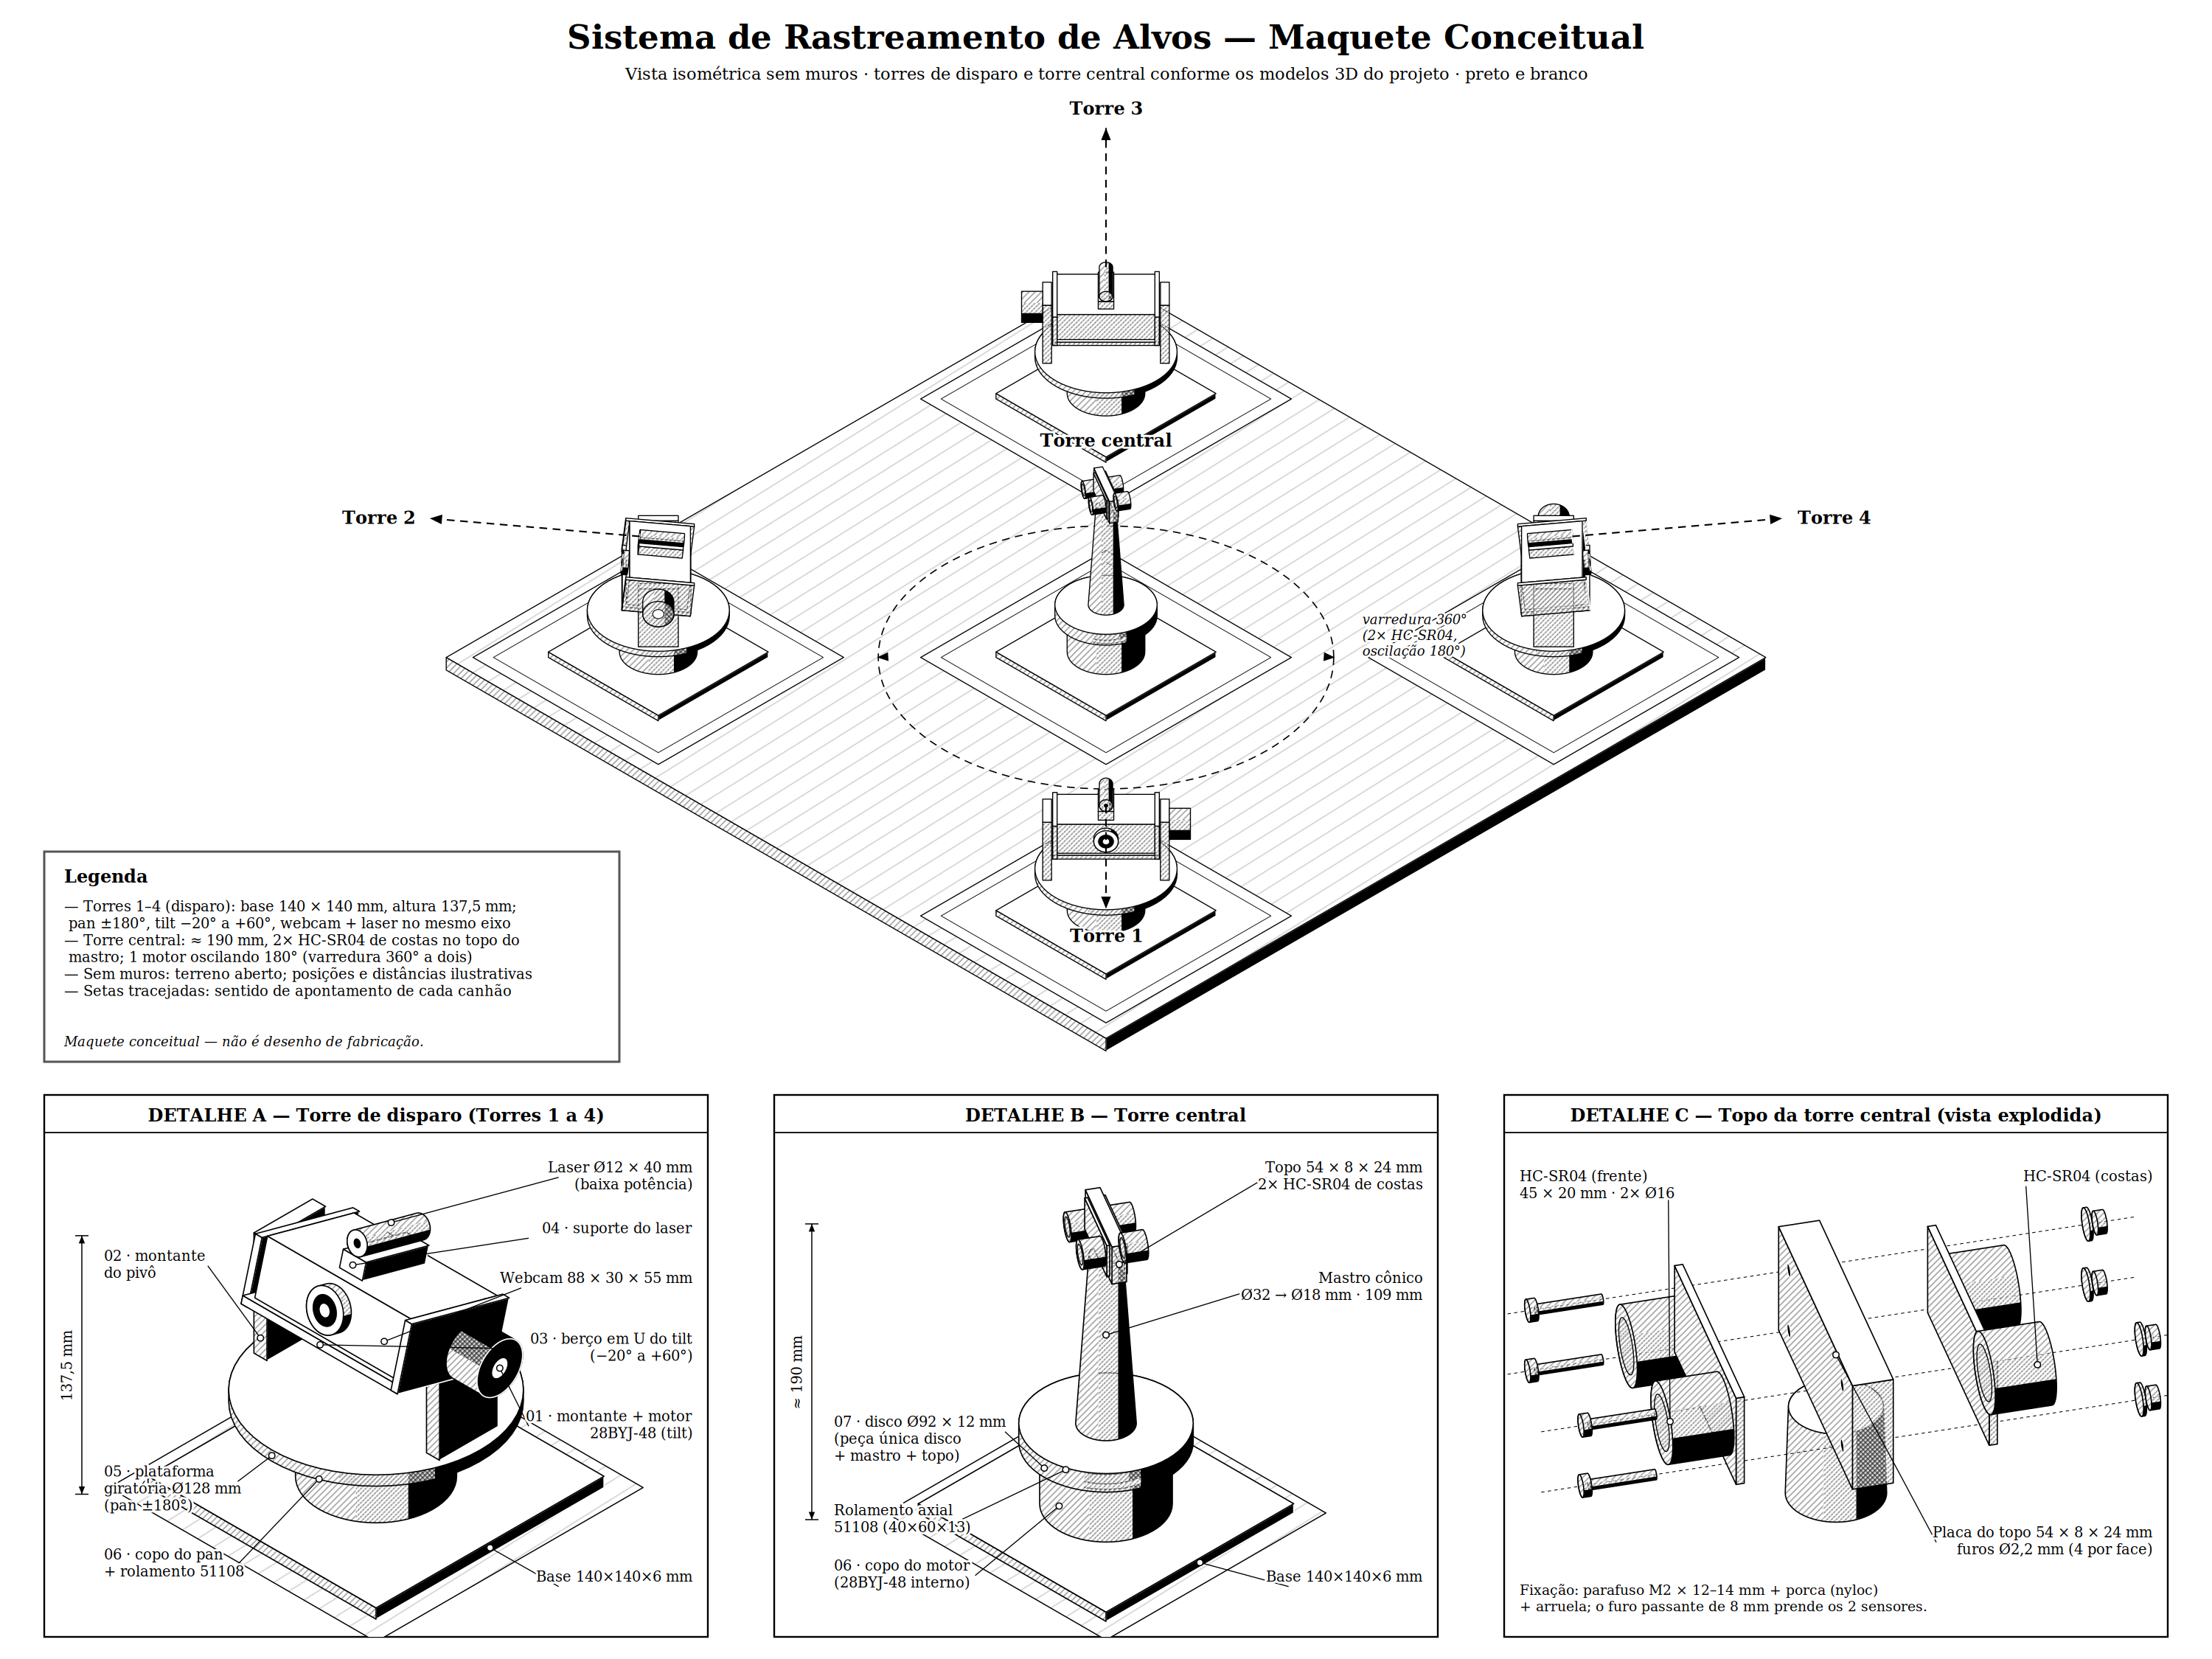
\includegraphics[width=\textwidth]{maquete_torres_isometrica.png}
  \caption{Maquete conceitual do arranjo das cinco torres (vista isométrica): quatro torres de disparo e a torre central com varredura de 360° (dos autores).}
\end{figure}

\subsubsection{Módulo de visão}

% CONFIRMAR: número de câmeras (quatro) e resolução (720p) -- não há registro desses valores no
% código nem na documentação do repositório.
O módulo de visão utiliza \grifo{quatro câmeras de 720p} conectadas por USB ao computador, associadas aos
quadrantes do radar, e processa os quadros de vídeo (\textit{frames}) para \grifo{classificar o alvo por
sua cor, formato e tamanho}. Cada quadro capturado é entregue já decodificado à detecção, que executa
localmente um modelo YOLO26, na variante nano, em formato ONNX, para propor as regiões candidatas
da imagem. Cada
candidata é então comparada ao perfil do alvo previamente cadastrado -- definido por cor, formato e
tamanho, e opcionalmente por fotos de referência recortadas no objeto de interesse. Havendo foto de
referência, a comparação combina um histograma de matiz e saturação com uma grade espacial de cor
média, usados como assinatura do objeto; na ausência de foto, o critério recai sobre a fração de
pixels com a cor cadastrada e sobre a classificação de formato. Quando o detector não propõe nenhuma
caixa com a cor do perfil, as regiões candidatas passam a ser propostas por segmentação de cor, como
último recurso na ordenação de candidatos.

\parecerAjuste{Mesma observação da Seção C.2: "quatro câmeras de 720p" não está registrado no
código nem na documentação técnica -- torne explícito se é decisão de projeto ou aspiração. O
trecho "classificar o alvo por sua cor, formato e tamanho" depende de uma técnica de visão
computacional clássica (classificação por cor/forma/tamanho) cuja referência bibliográfica ainda
não foi preenchida no \texttt{.tex} (comentário "PREENCHER" na Seção 2.1) -- resolver a citação
antes da entrega, já que é a base teórica de um componente central do sistema.}

O envio das informações resultantes ao Arduino, para guiar o apontamento da torre (movimentos de pan
e tilt), foi projetado mas ainda não está implementado: o protocolo serial atual não possui comando
de apontamento, e a fusão entre a posição estimada pela visão e a distância medida pelos sensores
ultrassônicos permanece como etapa planejada. Como o hardware ainda não foi montado, a validação
funcional descrita neste trabalho foi feita por simulação, e nenhum resultado de campo é relatado.

\subsubsection{Fluxo operacional}

Em operação, o sistema segue estas etapas: (1) o Arduino varre o ambiente com os dois sensores
ultrassônicos e envia ângulo e distância à aplicação; (2) a aplicação converte cada leitura em
posição cartesiana, determina o quadrante, exibe o alvo no radar e registra a detecção; (3) em
paralelo, as câmeras fornecem quadros de vídeo, e o módulo de visão classifica o alvo por cor,
formato e tamanho; (4) a aplicação seleciona, entre as torres armadas disponíveis, a mais adequada
para o alvo, priorizando as do mesmo quadrante e, entre elas, a de menor distância euclidiana (por
proximidade, alvo a alvo); (5) o comando é enviado ao Arduino, que aciona a torre selecionada;
(6) o acionamento demonstrativo (laser de baixa potência ou LED) só ocorre respeitando a distância
mínima de segurança e as demais regras de segurança configuráveis do sistema; (7) toda ação
executada é registrada em auditoria.

A seleção de torre e o acionamento dependem do modo de operação escolhido pelo operador, em um
modelo de três níveis: no primeiro, os alvos são apenas detectados e exibidos; no segundo,
acrescenta-se a seleção automática da torre, sem acionamento; no terceiro, acrescenta-se o
acionamento demonstrativo automático. Quando a regra de segurança reprova um acionamento, ele é
bloqueado e o motivo é registrado no console de eventos.

\begin{figure}[htbp]
  \centering
  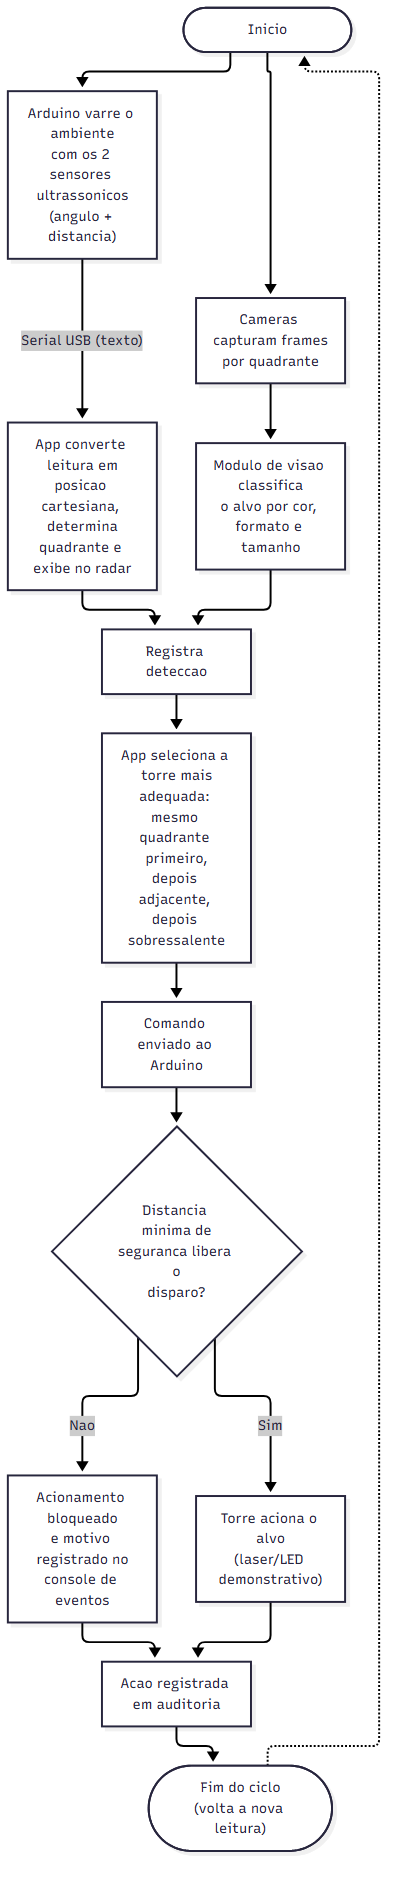
\includegraphics[height=0.82\textheight,width=\textwidth,keepaspectratio]{Fluxo_Operacional.png}
  \caption{Fluxograma do fluxo operacional do RadarTorres, da leitura dos sensores ao registro em
  auditoria (dos autores).}
\end{figure}


\subsubsection{Controlador neuroevolutivo: heurística e rede neural combinadas}
\label{sec:controlador-hibrido-inicio}

O passo (4) do fluxo operacional -- escolher, entre as torres armadas disponíveis, a mais adequada
para cada alvo, e decidir o instante do acionamento -- é resolvido no RadarTorres pela combinação
de dois mecanismos de natureza distinta: uma \textbf{heurística} determinística, escrita como regras
explícitas de engenharia, e uma \textbf{rede neural} \textit{feedforward}, cujo comportamento é
aprendido por um algoritmo evolutivo próprio, sem biblioteca de aprendizado de máquina. Ambos
coexistem no mesmo controlador híbrido, e é essa combinação -- não cada mecanismo isoladamente --
que determina tanto o comportamento em produção quanto o que é efetivamente treinado.

A heurística é um conjunto de regras fixas, escritas e revisáveis por engenharia, cujo resultado
para uma mesma entrada é sempre o mesmo. No RadarTorres ela resolve, em cascata, três camadas de
prioridade na seleção da torre: primeiro considera apenas as torres livres do próprio quadrante do
alvo; na ausência de candidata, estende-se às torres de quadrante adjacente cujo quadrante de
origem não tenha outro alvo concorrente; por fim, na ausência de qualquer uma das duas, recorre a
qualquer torre livre restante, de modo que nenhum alvo fique sem cobertura. Cada camada carrega um
fator numérico (1,0; 0,5; ou 0,0) que soma-se diretamente à pontuação da candidata. A heurística
também impõe cinco regras de segurança e refinamento, cada uma ativável individualmente no painel de
Configurações: anti-oscilação, que evita trocar de torre por uma diferença de pontuação dentro de
uma margem de empate; priorização por urgência, que permite a um alvo muito próximo da base "tomar"
a torre de um alvo mais distante; corredor de tiro, que descarta candidatas cuja linha de disparo
atravesse uma zona morta ativa; balanceamento de carga, que prefere, entre torres empatadas, a
usada com menor frequência na sessão; e predição de trajetória, que projeta a posição futura do
alvo para calcular o ângulo de mira com antecedência de poucos décimos de segundo. Por fim, a
heurística impõe dois limites absolutos ao disparo, nunca delegados à rede: um tempo mínimo de mira
de 0,3 s e um limiar mínimo de certeza de identificação do alvo
(\texttt{LimiarConfiancaDisparoPercentual}), abaixo do qual o disparo é recusado independentemente
de qualquer outra avaliação.

\parecerPergunta{Os limites de segurança (0,3s de mira, certeza mínima) são calibrados para o
ambiente SIMULADO. Já foi testado se esses limites fazem sentido físico para sensores ultrassônicos
e câmeras reais, nunca calibrados com dados de campo?}

A rede neural, por sua vez, não decide essas regras de segurança nem a cascata de camadas -- ela
decide apenas a escolha fina \textit{dentro} do espaço já validado pela heurística. É uma rede
\textit{feedforward} totalmente conectada, implementada do zero (sem biblioteca de aprendizado de
máquina), com arquitetura de 7 entradas, uma camada oculta de 8 neurônios e 2 saídas, com ativação
tanh em todas as camadas. As sete entradas -- todas normalizadas no intervalo $[0,1]$ ou
equivalente -- são a distância normalizada ao alvo, dois indicadores binários de quadrante (mesmo
quadrante e quadrante adjacente), o ângulo de mira normalizado, a velocidade normalizada do alvo, o
tempo normalizado em que o alvo está detectado sem ter sido abatido (sinal acrescentado para dar à
rede contexto sobre hesitação própria) e o
próprio fator da camada heurística vigente, usado como sinal de contexto. As duas saídas são um
ajuste de pontuação, somado à pontuação heurística da candidata, e um valor de confiança de
disparo, cujo sinal positivo autoriza o acionamento. Os pesos e vieses da rede -- 82 parâmetros, no
total, para essa arquitetura -- não são ajustados por retropropagação, mas evoluídos por um
algoritmo genético: cada genoma é um vetor plano desses 82 números, a população evolui por seleção
por torneio, \textit{crossover} uniforme, mutação gaussiana e elitismo, e o genoma final é
embutido na aplicação como um vetor de pesos fixo, sem qualquer etapa de treinamento em tempo de
execução.

\parecerElogio{Excelente correspondência verificada entre texto e código: arquitetura [6,8,2], 74
parâmetros, seleção por torneio de 3, crossover uniforme, mutação gaussiana (Box-Muller),
elitismo -- tudo conferido linha a linha em \texttt{RedeNeural.cs} e \texttt{AlgoritmoGenetico.cs}
e batendo exatamente com o relatado. Subseção tecnicamente mais confiável do artigo.}

A combinação entre os dois mecanismos é, portanto, sequencial e hierárquica, nunca uma mistura
indiferenciada: a heurística primeiro filtra quais torres são elegíveis e calcula as
\textit{features} de entrada (quadrante, ângulo, fator de camada); a rede neural, em seguida,
pondera essa pontuação dentro do subconjunto já validado, decidindo qual candidata específica
vence o empate fino que a heurística, por si só, não resolveria com a mesma sensibilidade; e, por
fim, a heurística volta a atuar como filtro de segurança sobre a decisão de disparo, vetando
qualquer autorização da rede que viole o tempo mínimo de mira, a certeza mínima ou uma zona morta
ativa. Essa hierarquia tem uma consequência deliberada para o pior caso: uma generalização
imperfeita da rede nunca produz uma decisão arbitrária, porque toda saída da rede continua restrita
ao espaço de candidatas e ao conjunto de disparos já pré-aprovados pela heurística -- no limite, o
sistema regride ao comportamento puramente heurístico, nunca a um erro fora de controle.

Esse acoplamento se reflete diretamente no treinamento do controlador. O algoritmo genético não
avalia a rede neural isolada: avalia o comportamento do \texttt{ControladorHibrido} completo --
heurística e rede juntas -- em episódios simulados de 45 s, com as torres reais do projeto, alvos
nascendo na borda de um mundo circular e avançando em direção à base. O fitness de cada genoma soma
recompensas por abate (maiores quanto mais longe da base o alvo é interceptado) e penalidades por
alvo que escapa ou cruza um ponto de perda sem decisão, de modo que o genoma é pressionado a
aprender a operar bem \textit{dentro} das restrições que a heurística já impõe, e não a contorná-las
-- não há genoma "vencedor" que dispare fora da zona morta ou abaixo da certeza mínima, porque essas
decisões nunca chegam a ser avaliadas como tal pelo ambiente de treino. Essa mesma dependência, no
entanto, também é o ponto mais sensível do processo: como o fitness depende inteiramente do
comportamento simulado, qualquer premissa equivocada no ambiente de treino se propaga,
silenciosamente, para o genoma evoluído. Foi exatamente esse o caso identificado e corrigido neste
trabalho -- a certeza de identificação do alvo era sorteada uma única vez, no nascimento, e nunca
era atualizada, de modo que cerca de 70\% dos alvos simulados nasciam permanentemente abaixo do
limiar mínimo de disparo e jamais podiam ser abatidos, independentemente da qualidade do genoma, o
que mascarava qualquer evolução real sob a aparência de estagnação. A correção -- fazer a certeza
crescer com o tempo de observação do alvo, como ocorreria com uma câmera real acumulando quadros --
e o alinhamento posterior dos parâmetros de alcance de mira e de limiar de certeza usados no treino
com os mesmos valores configuráveis em produção (\texttt{ConfiguracoesAplicativo.AlcanceMiraMetros},
\texttt{LimiarConfiancaDisparoPercentual}) ilustram, em conjunto, por que a fidelidade do ambiente
simulado ao comportamento do sistema real é, para um controlador neuroevolutivo, tão determinante
para o resultado do treinamento quanto a própria arquitetura da rede ou os hiperparâmetros da busca
genética.

\parecerElogio{A melhor contribuição empírica do artigo: achado real, com commit (\texttt{a02d46a})
e efeito quantificado (Tabela 1). Verificado pela banca como consistente com a mensagem de commit
real do repositório.}

\begin{figure}[htbp]
  \centering
  \resizebox{\textwidth}{!}{%
  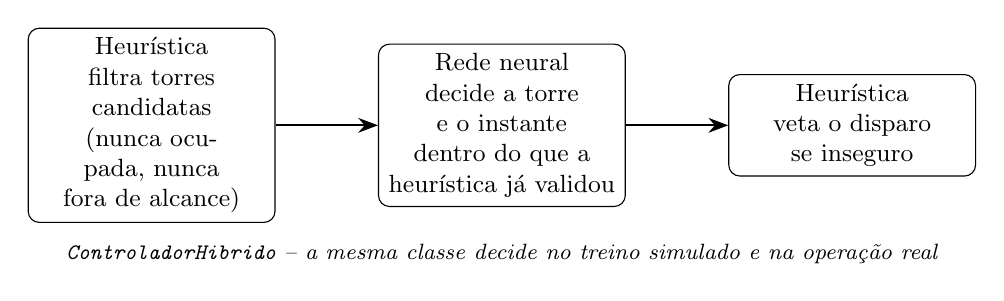
\begin{tikzpicture}[
      node distance=1.1cm and 1.3cm,
      box/.style={draw, rounded corners, align=center, minimum height=1.1cm, text width=2.9cm,
        font=\small},
      arr/.style={-{Stealth[length=2.5mm]}, thick}
    ]
    \node[box] (filtra) {Heurística\\filtra torres candidatas\\(nunca ocupada, nunca fora de alcance)};
    \node[box, right=of filtra] (decide) {Rede neural\\decide a torre e o instante\\dentro do que a
      heurística já validou};
    \node[box, right=of decide] (veta) {Heurística\\veta o disparo\\se inseguro};
    \draw[arr] (filtra) -- (decide);
    \draw[arr] (decide) -- (veta);
    \node[below=0.35cm of decide, font=\footnotesize\itshape] {\texttt{ControladorHibrido} -- a
      mesma classe decide no treino simulado e na operação real};
  \end{tikzpicture}%
  }
  \caption{Fluxo de decisão do controlador híbrido: a heurística determinística filtra e, ao final,
  veta; a rede neural decide apenas dentro do espaço já validado (dos autores).}
\end{figure}

\subsubsection{Análise experimental de hiperparâmetros: população e neurônios ocultos}
\label{sec:experimento-hiperparametros}

Para justificar tecnicamente a escolha dos hiperparâmetros do algoritmo genético com dados reais de
treinamento, em vez de apenas por convenção, foi conduzido um experimento controlado com as seis
combinações do produto cartesiano entre três tamanhos de população (30, 60 e 120 indivíduos) e duas
arquiteturas de rede (4 e 16 neurônios na camada oculta, mantendo fixas as 7 entradas e as 2 saídas
descritas na Seção~\ref{sec:controlador-hibrido-inicio}). Cada uma das seis combinações foi treinada
isoladamente por exatamente 300 gerações, com a mesma função de fitness, os mesmos cenários táticos
obrigatórios (\texttt{CatalogoCenarios.TodosComScript}) e a mesma taxa de mutação (0,08) do
treinamento padrão -- apenas a população e a arquitetura variaram entre as seis execuções, de modo a
isolar o efeito desses dois hiperparâmetros e manter a comparação justa. As seis execuções usaram o
mesmo \texttt{AmbienteTreinamento}/\texttt{AlgoritmoGenetico} que treina o controlador em produção,
sem nenhum dado simulado ou estimado manualmente; o resultado de cada combinação -- população,
gerações executadas, neurônios ocultos, fitness final do melhor indivíduo e data/hora -- foi
persistido na tabela \texttt{experimentos\_hiperparametros} (ver Seção~\ref{sec:modelo-dados}),
consultável na própria tela de Treinamento do Controlador.

\begin{table}[htbp]
  \centering
  \caption{Fitness final (melhor indivíduo, geração 300) das seis combinações de população ×
  neurônios ocultos, com todos os demais parâmetros de treinamento mantidos fixos.}
  \label{tab:experimento-hiperparametros}
  \small
  \renewcommand{\arraystretch}{1.2}
  \begin{tabular}{p{2.4cm}p{3.0cm}p{2.2cm}p{3.0cm}}
    \hline
    \textbf{População} & \textbf{Neurônios ocultos} & \textbf{Gerações} & \textbf{Fitness final} \\
    \hline
    30  & 4  & 300 & 49,81 \\
    60  & 4  & 300 & \textbf{52,19} \\
    120 & 4  & 300 & 49,81 \\
    30  & 16 & 300 & 49,81 \\
    60  & 16 & 300 & 49,81 \\
    120 & 16 & 300 & 49,81 \\
    \hline
  \end{tabular}
\end{table}

O resultado mais evidente da Tabela~\ref{tab:experimento-hiperparametros} não é qual combinação
"venceu", mas o quanto as seis convergiram para o mesmo valor: cinco das seis execuções
estabilizaram-se em exatamente 49,81 de fitness ao final das 300 gerações, e apenas a combinação de
população 60 com 4 neurônios ocultos escapou desse platô, ainda que por uma margem pequena (52,19).
Esse padrão é mais consistente com as seis execuções \grifo{convergindo para o mesmo ótimo local
acessível} dentro do horizonte de 300 gerações -- possivelmente próximo do comportamento da heurística pura, com
um ajuste de rede apenas marginal -- do que com um efeito forte e diferenciado de população ou
arquitetura sobre a qualidade final do controlador. Em outras palavras, dentro do horizonte testado,
nem aumentar a população (de 30 para 120 indivíduos) nem aumentar a camada oculta (de 4 para 16
neurônios) produziu, isoladamente, um controlador mensuravelmente melhor -- sinal de que o fator
limitante do treinamento, nesse horizonte, é provavelmente o número de gerações, não a capacidade da
rede nem o tamanho da amostra avaliada por geração.

\parecerGrave{PROBLEMA CRÍTICO (ver Seções C.1 e E.1 do parecer). A banca inspecionou
\texttt{ExecutorExperimentosHiperparametros.cs} e \texttt{AmbienteTreinamento.AvaliarFitness}: as
seeds de avaliação dependem apenas do número da geração (\texttt{geracaoAtual * 1000 + i}), não da
configuração, e a maioria dos episódios por avaliação de fitness usa cenários roteirizados
(\texttt{CatalogoCenarios.TodosComScript}) com seed fixa 0 -- idênticos entre as seis combinações, a
cada geração. Isso é uma explicação mecânica muito mais parcimoniosa para "5 de 6 execuções em
exatamente 49,81" do que "convergência coincidente para o mesmo ótimo local": genomas que convergem
para a mesma estratégia produzem trajetórias bit-a-bit idênticas nos componentes determinísticos do
ambiente. O texto grifado acima não menciona essa característica do desenho experimental.
Correção sugerida: acrescentar um parágrafo reconhecendo que parte da avaliação é determinística
por configuração do experimento, e que isso é uma explicação alternativa plausível -- talvez mais
provável -- para a convergência exata observada.}

Essa leitura em termos de ótimo local precisa, porém, de uma ressalva importante sobre o próprio
desenho do experimento: parte da avaliação de fitness em cada geração é determinística por
configuração, não apenas por convergência das seis populações. As seeds usadas para gerar os
episódios de avaliação dependem só do número da geração (\texttt{geracaoAtual * 1000 + i}), e não
da combinação de população/arquitetura sendo testada; além disso, a maioria dos episódios de cada
avaliação usa cenários roteirizados de seed fixa (\texttt{CatalogoCenarios.TodosComScript}),
idênticos entre as seis execuções a cada geração. Isso significa que, se duas combinações
convergirem para a mesma estratégia de decisão, elas tendem a produzir trajetórias
bit-a-bit idênticas nos componentes determinísticos do ambiente de avaliação -- uma explicação
mecânica, derivada diretamente do desenho experimental, ao menos tão plausível quanto a
convergência para o mesmo ótimo local acessível para explicar por que exatamente 49,81 de fitness
se repete em cinco das seis combinações. As duas explicações não são mutuamente exclusivas: é
plausível que as cinco combinações estejam, de fato, perto do mesmo ótimo local -- o que tornaria o
determinismo das seeds compatível, e não concorrente, com esse platô -- mas o desenho atual do
experimento não permite distinguir entre as duas hipóteses.

Duas ressalvas são necessárias para a correta leitura deste experimento, na mesma linha das já
apontadas na Seção~\ref{sec:procedimentos-metodologicos} para o treinamento do controlador em geral.
Primeiro, cada combinação corresponde a uma única execução (uma trajetória de evolução), não a uma
média de repetições independentes; a diferença entre 49,81 e 52,19 é pequena demais, com uma amostra
de tamanho 1 por combinação, para ser atribuída com confiança ao hiperparâmetro em si, em vez de à
variação natural entre execuções de um algoritmo estocástico. Segundo, o horizonte de 300 gerações foi
escolhido para manter o experimento executável em poucos minutos (entre 9,3 e 33,4 segundos por
combinação, 123,4 segundos no total para as seis, medidos no mesmo processo que gerou a
Tabela~\ref{tab:experimento-hiperparametros}), não necessariamente para captar a convergência completa
de cada configuração -- o próprio platô compartilhado por cinco das seis combinações sugere que mais
gerações poderiam, ainda, diferenciá-las entre si.

\parecerElogio{Transparência genuína e rara: o texto reconhece explicitamente n=1 por combinação e
o horizonte curto de gerações, em vez de apresentar a tabela sem ressalvas. Isso não substitui a
investigação da causa determinística (ver comentário acima), mas é um mérito de honestidade
científica.}

Com essas ressalvas, a conclusão prática deste experimento para a escolha de hiperparâmetros do
RadarTorres é de custo-benefício, não de desempenho: como nenhuma das combinações testadas superou as
demais de forma consistente, não há evidência, neste horizonte de treinamento, que justifique o custo
computacional adicional de uma população maior (120 indivíduos, cerca de 3,2$\times$ o tempo de
execução de uma população de 30 nesta amostra) ou de uma camada oculta maior (16 neurônios, mais que o
dobro dos parâmetros treináveis de uma rede com 4). A arquitetura de produção -- população de 60
indivíduos e 8 neurônios na camada oculta, intermediária às duas arquiteturas aqui testadas --
permanece, portanto, \grifo{uma escolha razoável dentro da faixa investigada}, mas este experimento evidencia
a necessidade de uma repetição futura com mais gerações e múltiplas sementes por combinação antes de
se afirmar que ela é estritamente superior às demais, trabalho futuro já na mesma linha da ressalva
geral sobre a fidelidade do ambiente de treino feita na Seção~\ref{sec:procedimentos-metodologicos}.

\parecerAjuste{Esta conclusão usa a AUSÊNCIA de uma combinação melhor (n=1 cada) para validar, por
omissão de alternativa, a configuração já em produção -- um raciocínio de "ausência de evidência
contrária" tratado quase como evidência a favor. É coerente com as ressalvas do parágrafo anterior,
mas vale deixar ainda mais explícito que isso NÃO é uma validação positiva da escolha de produção,
só a ausência (neste experimento limitado) de uma alternativa comprovadamente superior.}

\subsection{Diagrama de pacotes}

A organização interna da aplicação desktop foi documentada por meio de um diagrama de pacotes,
diagrama estrutural da UML que representa a divisão lógica do sistema em pacotes e as
dependências existentes entre eles, sem detalhar atributos ou métodos das classes neles contidas.
No RadarTorres, cada pacote corresponde a um \textit{namespace} do projeto
\texttt{RadarTorres.App}, coincidente com uma pasta do código-fonte, e o diagrama foi obtido
diretamente do código da \textit{branch} principal do repositório: cada seta representa ao menos
uma diretiva \texttt{using RadarTorres.App.*} (ou uma referência \texttt{clr-namespace} em XAML)
presente nos arquivos do pacote de origem, de modo que o diagrama descreve a estrutura efetivamente
implementada, e não apenas a pretendida.

\begin{figure}[htbp]
  \centering
  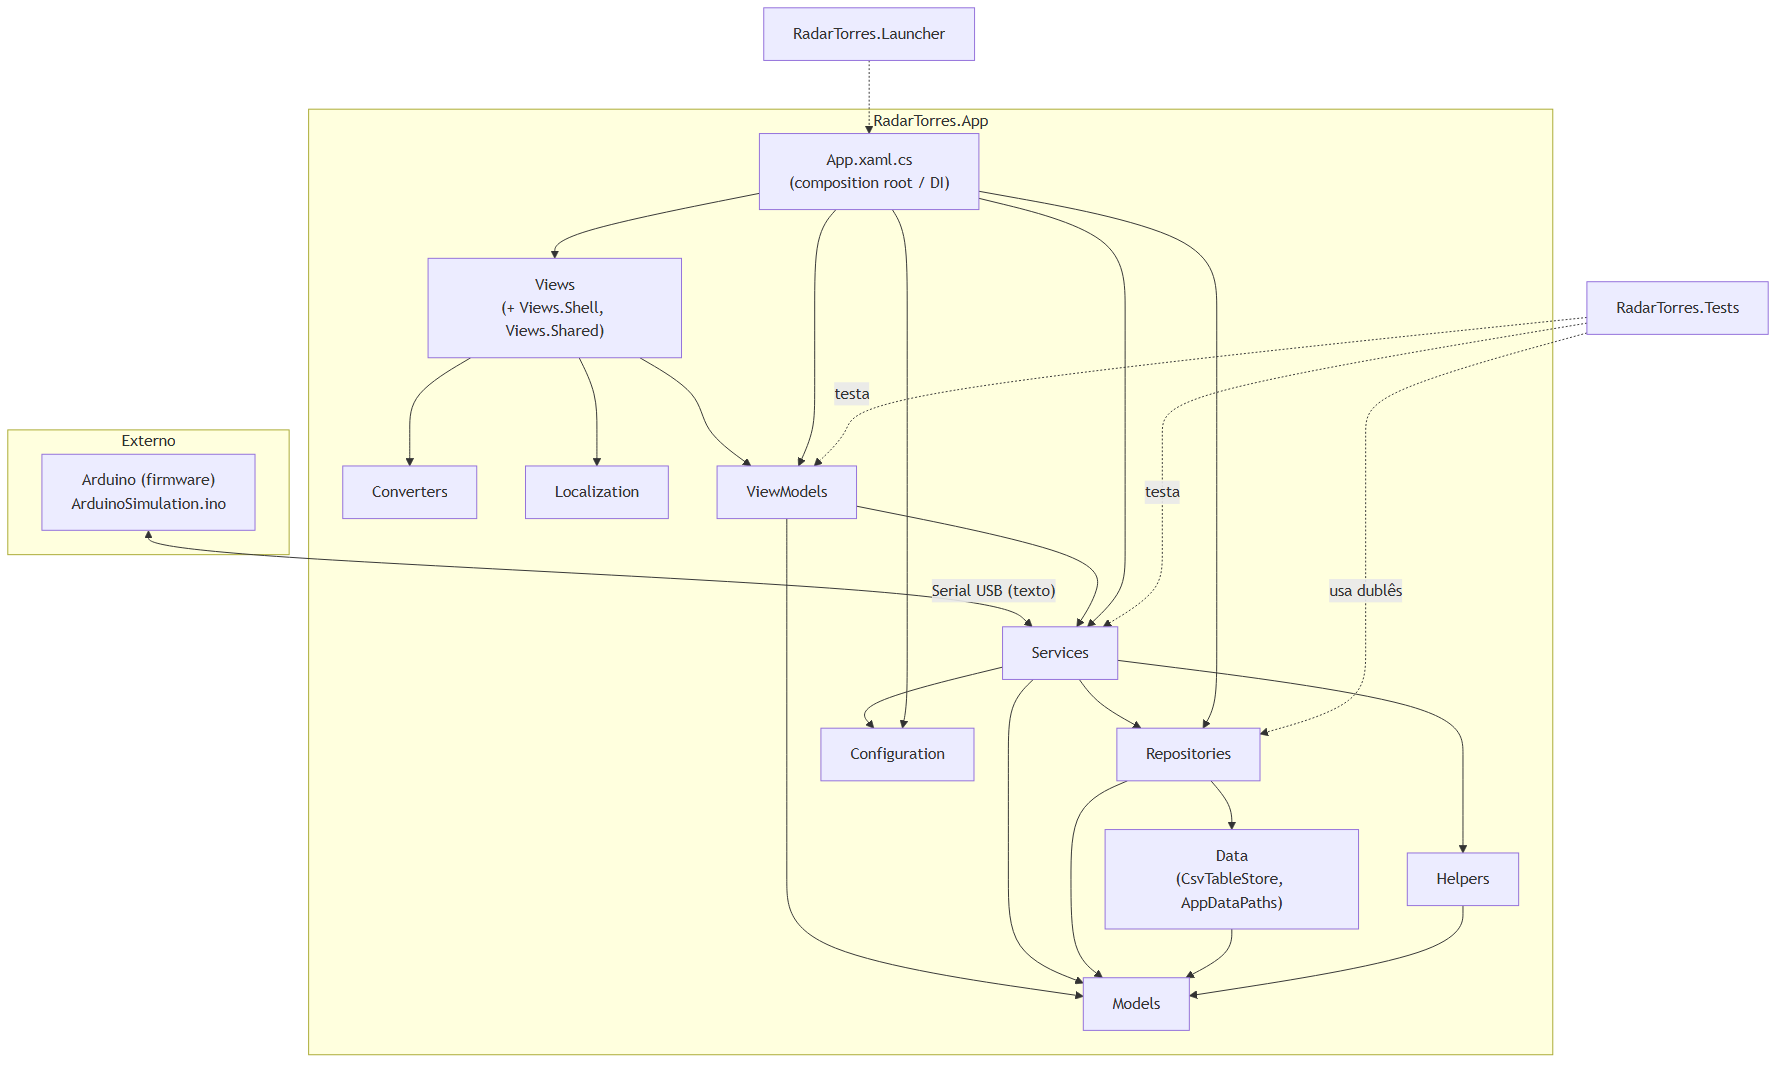
\includegraphics[width=\textwidth]{Diagrama_de_Pacotes.png}
  \caption{Diagrama de pacotes do RadarTorres. Setas em vermelho indicam dependências que formam
  ciclos (dos autores).}
\end{figure}

O fluxo principal de dependências segue a organização do padrão MVVM, de cima para baixo: Views
$\rightarrow$ ViewModels $\rightarrow$ Services $\rightarrow$ Repositories $\rightarrow$ Data
$\rightarrow$ Models. O pacote Models ocupa a posição mais estável do sistema -- todos os demais
dependem dele e ele não depende de nenhum outro --, o que é desejável para as entidades de
domínio, e a separação entre as interfaces de Repositories e a implementação em CSV do pacote Data
é o que viabiliza a futura migração para um banco relacional sem alterar ViewModels ou Services. A
construção do diagrama a partir do código revelou, também, dependências que formam ciclos entre
pacotes: o \texttt{NavigationService} importa \textit{namespaces} de Views para instanciar telas
(Services $\rightarrow$ Views, fechando o ciclo com Views $\rightarrow$ ViewModels $\rightarrow$
Services), e o \texttt{DataSeeder}, responsável pela carga inicial de dados, importa Models,
Repositories e Services (Data $\rightarrow$ Repositories/Services, fechando o ciclo com
Repositories/Services $\rightarrow$ Data). Confirmados em \texttt{NavigationService.cs} e
\texttt{DataSeeder.cs} no código atual, esses dois ciclos continuam presentes, mas a figura acima,
regenerada ao nível de pacote e não de classe, não os destaca visualmente -- ficam registrados
apenas neste parágrafo, em vez de perdidos. Eles não impedem o funcionamento da aplicação, pois
todos os pacotes pertencem ao mesmo \textit{assembly}, mas aumentam o acoplamento e dificultam
testes isolados e futuras separações em projetos distintos.

\parecerElogio{Reconhecimento honesto de um achado desfavorável (ciclos de dependência) que a
maioria dos TCCs omitiria -- mérito de rigor e transparência.}


\subsection{Modelo de dados}
\label{sec:modelo-dados}

A persistência do RadarTorres foi igualmente documentada por meio de um levantamento do modelo de
dados diretamente a partir do código-fonte já implementado. O protótipo não depende de um
servidor de banco de dados: utiliza \textbf{SQLite} (\texttt{Microsoft.Data.Sqlite}, arquivo único \texttt{radartorres.db} na
pasta de dados do usuário), com \texttt{PRAGMA foreign\_keys = ON} garantindo chaves estrangeiras
reais --
estágio mais avançado do que o modelo em CSV descrito em versões anteriores deste documento (ver
nota histórica adiante). O schema atual tem onze tabelas, listadas na Tabela~\ref{tab:tabelas-sqlite}:
sete cadastrais/de auditoria, já cobertas pelo levantamento em
\texttt{conteudo\_modelo\_banco\_dados.tex} (pasta \texttt{Banco\_de\_Dados} dos documentos
entregáveis), e quatro
exclusivas do treinamento neuroevolutivo, que persistem a evolução do controlador híbrido
(Seção~\ref{sec:controlador-hibrido-inicio}) entre execuções.

\begin{table}[htbp]
  \centering
  \caption{Tabelas do schema SQLite atual (\texttt{schema.sql} e os \texttt{Sqlite*Repository.cs}).}
  \label{tab:tabelas-sqlite}
  \small
  \renewcommand{\arraystretch}{1.2}
  \begin{tabular}{p{4.6cm}p{7.6cm}}
    \hline
    \textbf{Tabela} & \textbf{Finalidade} \\
    \hline
    \texttt{usuarios} & Contas de acesso, perfil (Administrador/Operador/Visualizador) e
    autenticação \\
    \texttt{objetos\_detectados} & Histórico de ocorrências de detecção (radar e câmera, por
    quadrante) \\
    \texttt{ocorrencia\_estados} & Auditoria das transições de estado de cada ocorrência
    (só inserção) \\
    \texttt{cameras} & Câmera responsável por cada quadrante (Q1--Q4) \\
    \texttt{acoes\_realizadas} & Auditoria de acionamentos efetivamente executados (só inserção) \\
    \texttt{modo\_atual\_torre} & Auditoria de troca de modo de operação (só inserção) \\
    \texttt{preferencias\_usuario} & Preferências de interface por usuário (tema, idioma,
    sidebar) \\
    \texttt{classificacoes\_alvo} & Classificação de perigo do alvo por velocidade estimada,
    vinculada a \texttt{objetos\_detectados} por FK \\
    \texttt{historico\_treinamento\_\allowbreak geracoes} & Fitness (melhor e médio) e contagem de
    alvos abatidos/escapados a cada geração do algoritmo genético \\
    \texttt{marcos\_fitness\_\allowbreak treinamento} & Agregado de fitness por bloco de gerações, para
    acompanhar a convergência do treino sem gravar geração a geração \\
    \texttt{instantaneos\_\allowbreak comportamento\_\allowbreak melhor\_gene} & Snapshot do comportamento do melhor
    indivíduo em marcos do treino: fitness, taxa de acerto, taxa de cobertura e o próprio genoma
    (JSON) \\
    \hline
  \end{tabular}
\end{table}

O modelo de dados atual (SQLite, 11 tabelas, chaves estrangeiras reais) é apresentado a seguir em
três grupos, por legibilidade: o núcleo de usuários e preferências (Figura~\ref{fig:der-usuarios}),
o núcleo de detecção, câmeras e auditoria (Figura~\ref{fig:der-cameras}) e as tabelas de
treinamento neuroevolutivo, independentes entre si (Figura~\ref{fig:der-treinamento}) -- diagramas
entidade-relacionamento levantados a partir do código-fonte do projeto.

\begin{figure}[htbp]
  \centering
  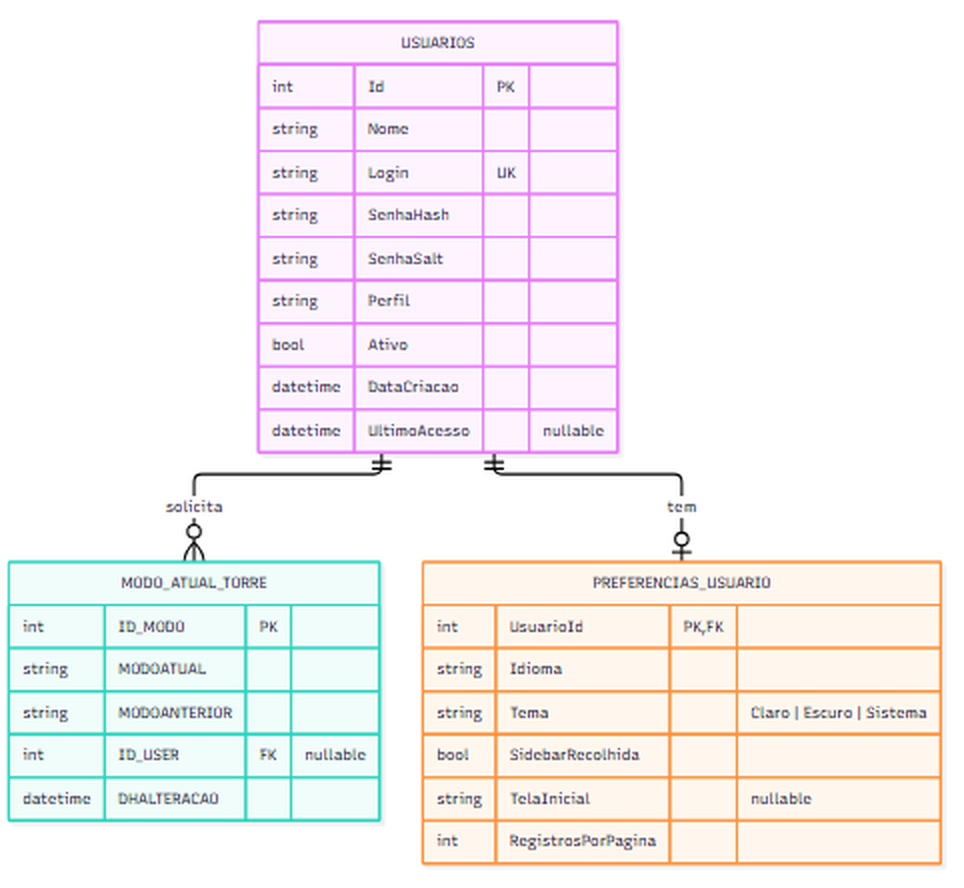
\includegraphics[width=0.85\textwidth]{DER_Usuarios_Modo_Preferencias.png}
  \caption{Núcleo de usuários: \texttt{usuarios}, \texttt{modo\_atual\_torre} e
  \texttt{preferencias\_usuario} (dos autores).}
  \label{fig:der-usuarios}
\end{figure}

\begin{figure}[htbp]
  \centering
  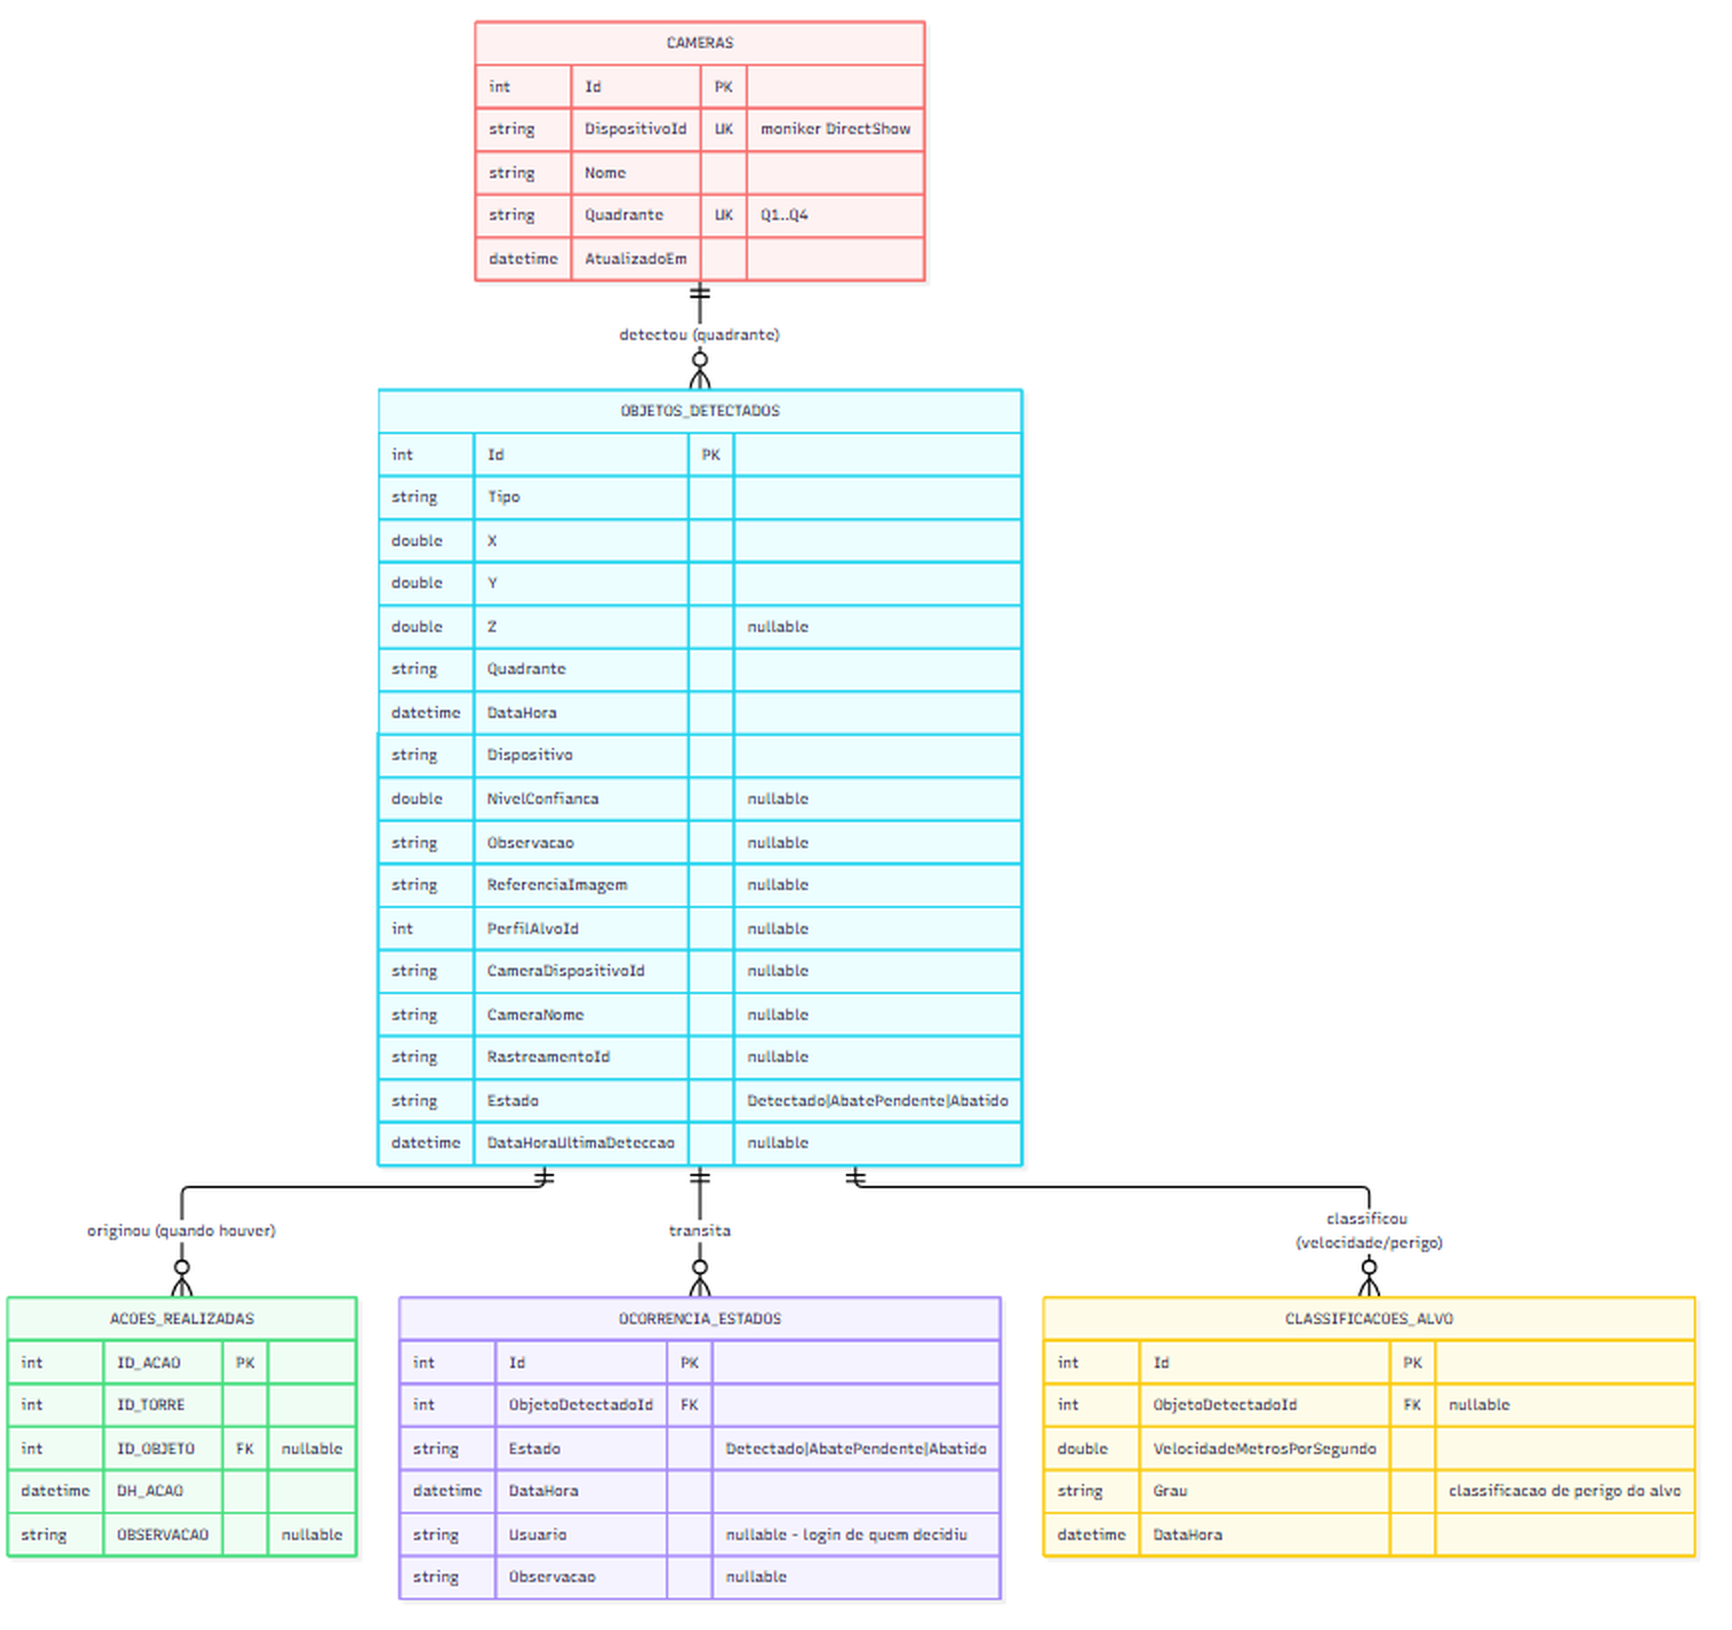
\includegraphics[width=\textwidth]{DER_Cameras_Objetos_Detectados.png}
  \caption{Núcleo de detecção e auditoria: \texttt{cameras}, \texttt{objetos\_detectados},
  \texttt{acoes\_realizadas}, \texttt{ocorrencia\_estados} e \texttt{classificacoes\_alvo} (dos
  autores).}
  \label{fig:der-cameras}
\end{figure}

\begin{figure}[htbp]
  \centering
  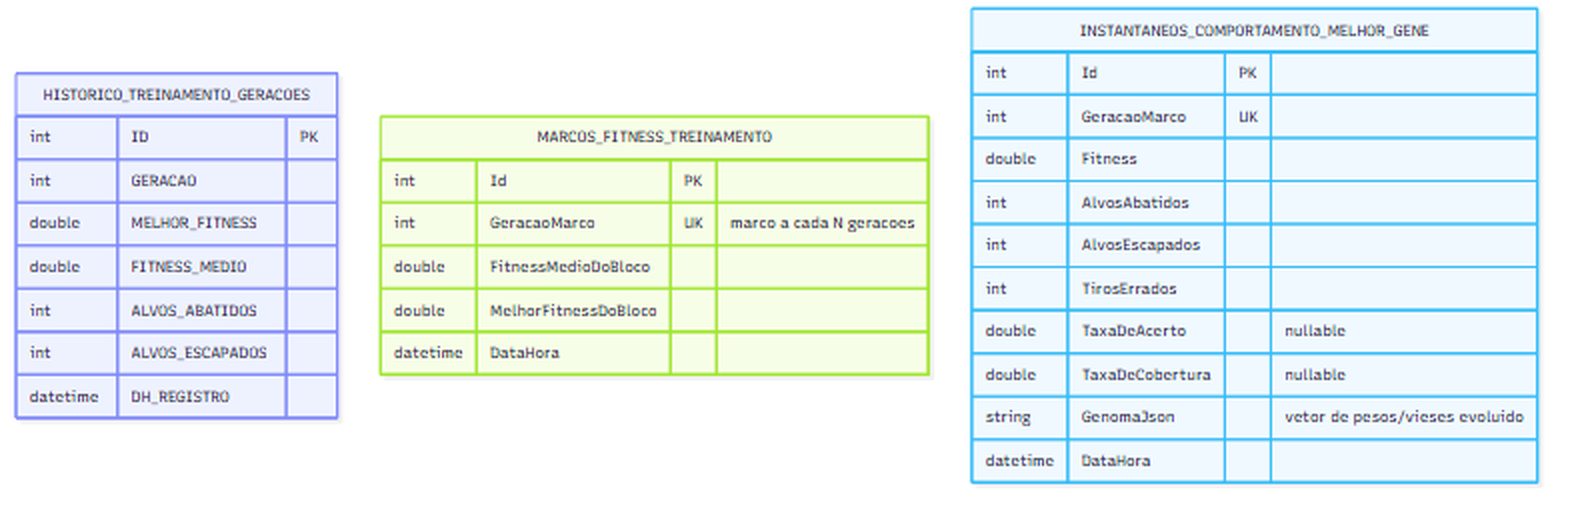
\includegraphics[width=\textwidth]{DER_Tabelas_Treinamento.png}
  \caption{Tabelas de treinamento neuroevolutivo -- séries temporais independentes entre si:
  \texttt{historico\_treinamento\_geracoes}, \texttt{marcos\_fitness\_treinamento} e
  \texttt{instantaneos\_comportamento\_melhor\_gene} (dos autores).}
  \label{fig:der-treinamento}
\end{figure}

\texttt{usuarios} se relaciona 1:1 com \texttt{preferencias\_usuario} (chave
\texttt{UsuarioId} $\rightarrow$ \texttt{usuarios.Id}) e 1:N com \texttt{modo\_atual\_torre}
(\texttt{ID\_USER} $\rightarrow$ \texttt{usuarios.Id}) -- em ambos os casos por chave estrangeira
real de inteiro, não mais por login em texto. \texttt{objetos\_detectados} se relaciona 1:N com
\texttt{acoes\_realizadas} (quando há alvo associado ao acionamento), com
\texttt{ocorrencia\_estados} (histórico de transição de estado) e com
\texttt{classificacoes\_alvo} (\texttt{ObjetoDetectadoId} $\rightarrow$
\texttt{objetos\_detectados.Id}); \texttt{cameras} se relaciona 1:N com
\texttt{objetos\_\allowbreak detectados} pelo quadrante monitorado. As quatro tabelas de treinamento não se relacionam por FK com as demais
nem entre si: são séries temporais independentes, cada uma identificada pelo número da geração
(\texttt{GERACAO}/\texttt{GeracaoMarco}) e pelo instante de registro, cobrindo da granularidade
mais fina (\texttt{historico\_treinamento\_geracoes}, uma linha por geração) à mais agregada
(\texttt{instantaneos\_comportamento\_melhor\_gene}, uma linha por marco, com o genoma completo em
JSON).

Como registro histórico do projeto, o modelo original em arquivos CSV tinha seis entidades (sem
\texttt{ChamadoAjuda}, removida do código) e nenhuma chave estrangeira real -- os vínculos entre
\texttt{Usuario} e \texttt{AcaoRealizada}/\texttt{ModoAtualTorre} eram feitos por login em texto. A
migração efetivamente realizada seguiu a proposta elaborada a partir desse modelo original para as
sete entidades que já existiam, mas foi além dela ao acrescentar as quatro tabelas de treinamento
neuroevolutivo, inexistentes na época em que a proposta foi desenhada.

\section{Conclusão}

Este trabalho descreveu o RadarTorres como um protótipo de rastreamento e seleção automática de
alvos construído sobre sensoriamento ultrassônico, visão computacional e um controlador híbrido
-- heurística determinística que filtra e veta, rede neural pequena que decide dentro do espaço já
validado, treinada por algoritmo genético. A contribuição mais original deste trabalho é empírica:
a identificação e correção, documentada por commit, de uma falha em que a certeza de identificação
do alvo era sorteada uma única vez e nunca atualizada, mantendo cerca de 70\% dos alvos
simulados permanentemente abaixo do limiar de disparo e mascarando a estagnação evolutiva sob a
aparência de um treino funcional. A Tabela~\ref{tab:fitness-antes-depois} (Seção anterior) quantifica
o efeito dessa correção: o fitness médio da população, estagnado em torno de 9 ao longo de 25.500
gerações antes da correção, passou a acompanhar de perto o fitness do melhor indivíduo depois dela,
e a cobertura de alvos disparáveis foi de uma fração minoritária para 100\% nas amostras
pós-correção.

As limitações do protótipo, discutidas ao longo do texto, concentram-se em três pontos: (i) o
hardware físico ainda não foi montado -- toda validação é feita em simulação, com modelos
(certeza de identificação, probabilidade de erro de disparo) assumidos e não calibrados com dados
de campo; (ii) a comunicação entre a visão computacional e o Arduino para guiar o apontamento de
pan/tilt foi projetada mas não implementada, permanecendo como integração pendente; e (iii) a
propriedade de projeto que limita o controlador híbrido, no pior caso, ao comportamento puramente
heurístico (nunca a uma decisão arbitrária da rede) ainda não foi submetida a validação em hardware
físico real.

Os trabalhos futuros identificados neste artigo são, portanto: montagem e validação do hardware
físico das cinco torres; implementação do comando de apontamento no protocolo serial e da fusão
entre a posição estimada pela visão e a distância ultrassônica; calibração dos modelos de certeza e
de erro de disparo com dados de campo, substituindo as premissas simuladas; extensão da seleção de
torre para a abordagem multiameaça da literatura de TEWA, hoje deixada de lado em favor da
abordagem por proximidade; e, caso a capacidade da rede se mostre o fator limitante do controlador
em vez dos hiperparâmetros da busca evolutiva, avaliação de uma arquitetura maior à luz dos
resultados de \citeonline{such2017deepneuroevolution}.

% ============================================================
% PARECER FINAL DA BANCA (Banca_TCC)
% ============================================================
\clearpage
\section*{Parecer final da banca (Banca\_TCC, revisão automatizada desta versão)}

\subsection*{Nota geral}

\textbf{$\approx 6{,}33/10$} -- ver tabela de critérios e justificativas completas em
\texttt{Parecer\_Banca\_TCC.pdf}, Seção B.

\subsection*{Coerência geral}

Trabalho tecnicamente competente, com uma contribuição empírica real e bem documentada (o bug de
certeza estática, Tabela~\ref{tab:fitness-antes-depois}) e uma honestidade metodológica consistente
sobre a ausência de hardware físico. O problema central que permanece é a mistura, sem sinalização
ao leitor, de afirmações com proveniência muito diferente: parte rastreável ao código linha a linha
(o controlador neuroevolutivo, Seção 2.3.5), parte admitidamente não confirmada em código nem em
documentação (projeto elétrico/estrutural, Seção 2.3.2, e parte do módulo de visão, Seção 2.3.3) --
o que contradiz diretamente a alegação de rastreabilidade total feita na Seção 2.2. Soma-se a leitura
interpretativa incompleta da Tabela~\ref{tab:experimento-hiperparametros} (Seção 2.3.6), que não
discute a causa determinística mais provável da convergência exata observada.

\textbf{Veredito}: APROVADO COM RESSALVAS -- os itens marcados
\textbf{\color{red!60!black}BANCA\_TCC -- PROBLEMA CRÍTICO/ALTO} nesta revisão precisam ser
resolvidos antes da entrega final/defesa; os marcados \textbf{AJUSTAR} são recomendados, mas não
impediriam a defesa.

\subsection*{Plano de correção priorizado}

\footnotesize
\begin{longtable}{|p{0.9cm}|p{6.3cm}|p{7.0cm}|}
\hline
\textbf{Prior.} & \textbf{Ação} & \textbf{Motivo} \\
\hline
\endhead
1 (máx.) & Discutir no texto a causa determinística provável da convergência exata na Tabela 2
(Seção 2.3.6) & Afeta diretamente a validade da conclusão mais recente e mais citada do artigo \\
\hline
2 (máx.) & Reconciliar a Seção 2.3.2 (elétrico/estrutural) e parte da 2.3.3 (visão) com a
documentação técnica real, ou sinalizar a incerteza no próprio PDF & Contradição direta com a
alegação metodológica central do artigo (Seção 2.2) \\
\hline
3 (alta) & Preencher a citação pendente sobre classificação por cor/forma/tamanho (comentário
"PREENCHER" na Seção 2.1) & Lacuna teórica central já identificada pelo próprio autor \\
\hline
4 (alta) & Versionar o genoma embutido (\texttt{genoma-controlador.json}) junto com a versão final
do artigo & O artefato citado no texto já diverge do estado atual do repositório \\
\hline
5 (média) & Completar o \texttt{.bib} com DOI/veículo/páginas, especialmente para as referências
centrais (Such 2017, Huang \& Ontañón 2020, Alshiekh 2017) & Abaixo do padrão mínimo de
rastreabilidade bibliográfica \\
\hline
6 (média) & Marcar explicitamente, na Tabela 1, qual célula é estimativa derivada vs. medição
direta & Evita confundir leitor sobre a natureza do número \\
\hline
7 (baixa) & Preencher o placeholder "Mestre em xxx pela xxx" no rodapé do orientador & Pendência
de formatação antes de qualquer submissão formal \\
\hline
8 (baixa) & Resolver \textit{overfull/underfull hboxes} remanescentes e remover macros de revisão
(\texttt{\textbackslash revmudar} etc.) não utilizadas & Polimento final de tipografia \\
\hline
\end{longtable}
\normalsize

O parecer completo (seções A a J, nota ponderada por critério, auditoria de referências e de
figuras/tabelas, e as perguntas que a banca provavelmente fará na defesa) está em
\texttt{Parecer\_Banca\_TCC.pdf}, gerado na mesma análise que originou estas marcações.

% ============================================================
% REFERÊNCIAS
% ============================================================
\bibliography{referencias}

\end{document}
